\section{PRECIPITATIONS}




IN general, the forecast of precipitations is more complicated than temperature, thus the scores are a little less good for this part especially the deterministic ones. 



\subsection{Deterministic Evaluation Metrics}

\subsubsection{Spearman rank correlation}

\begin{figure}[H]
	\centering
	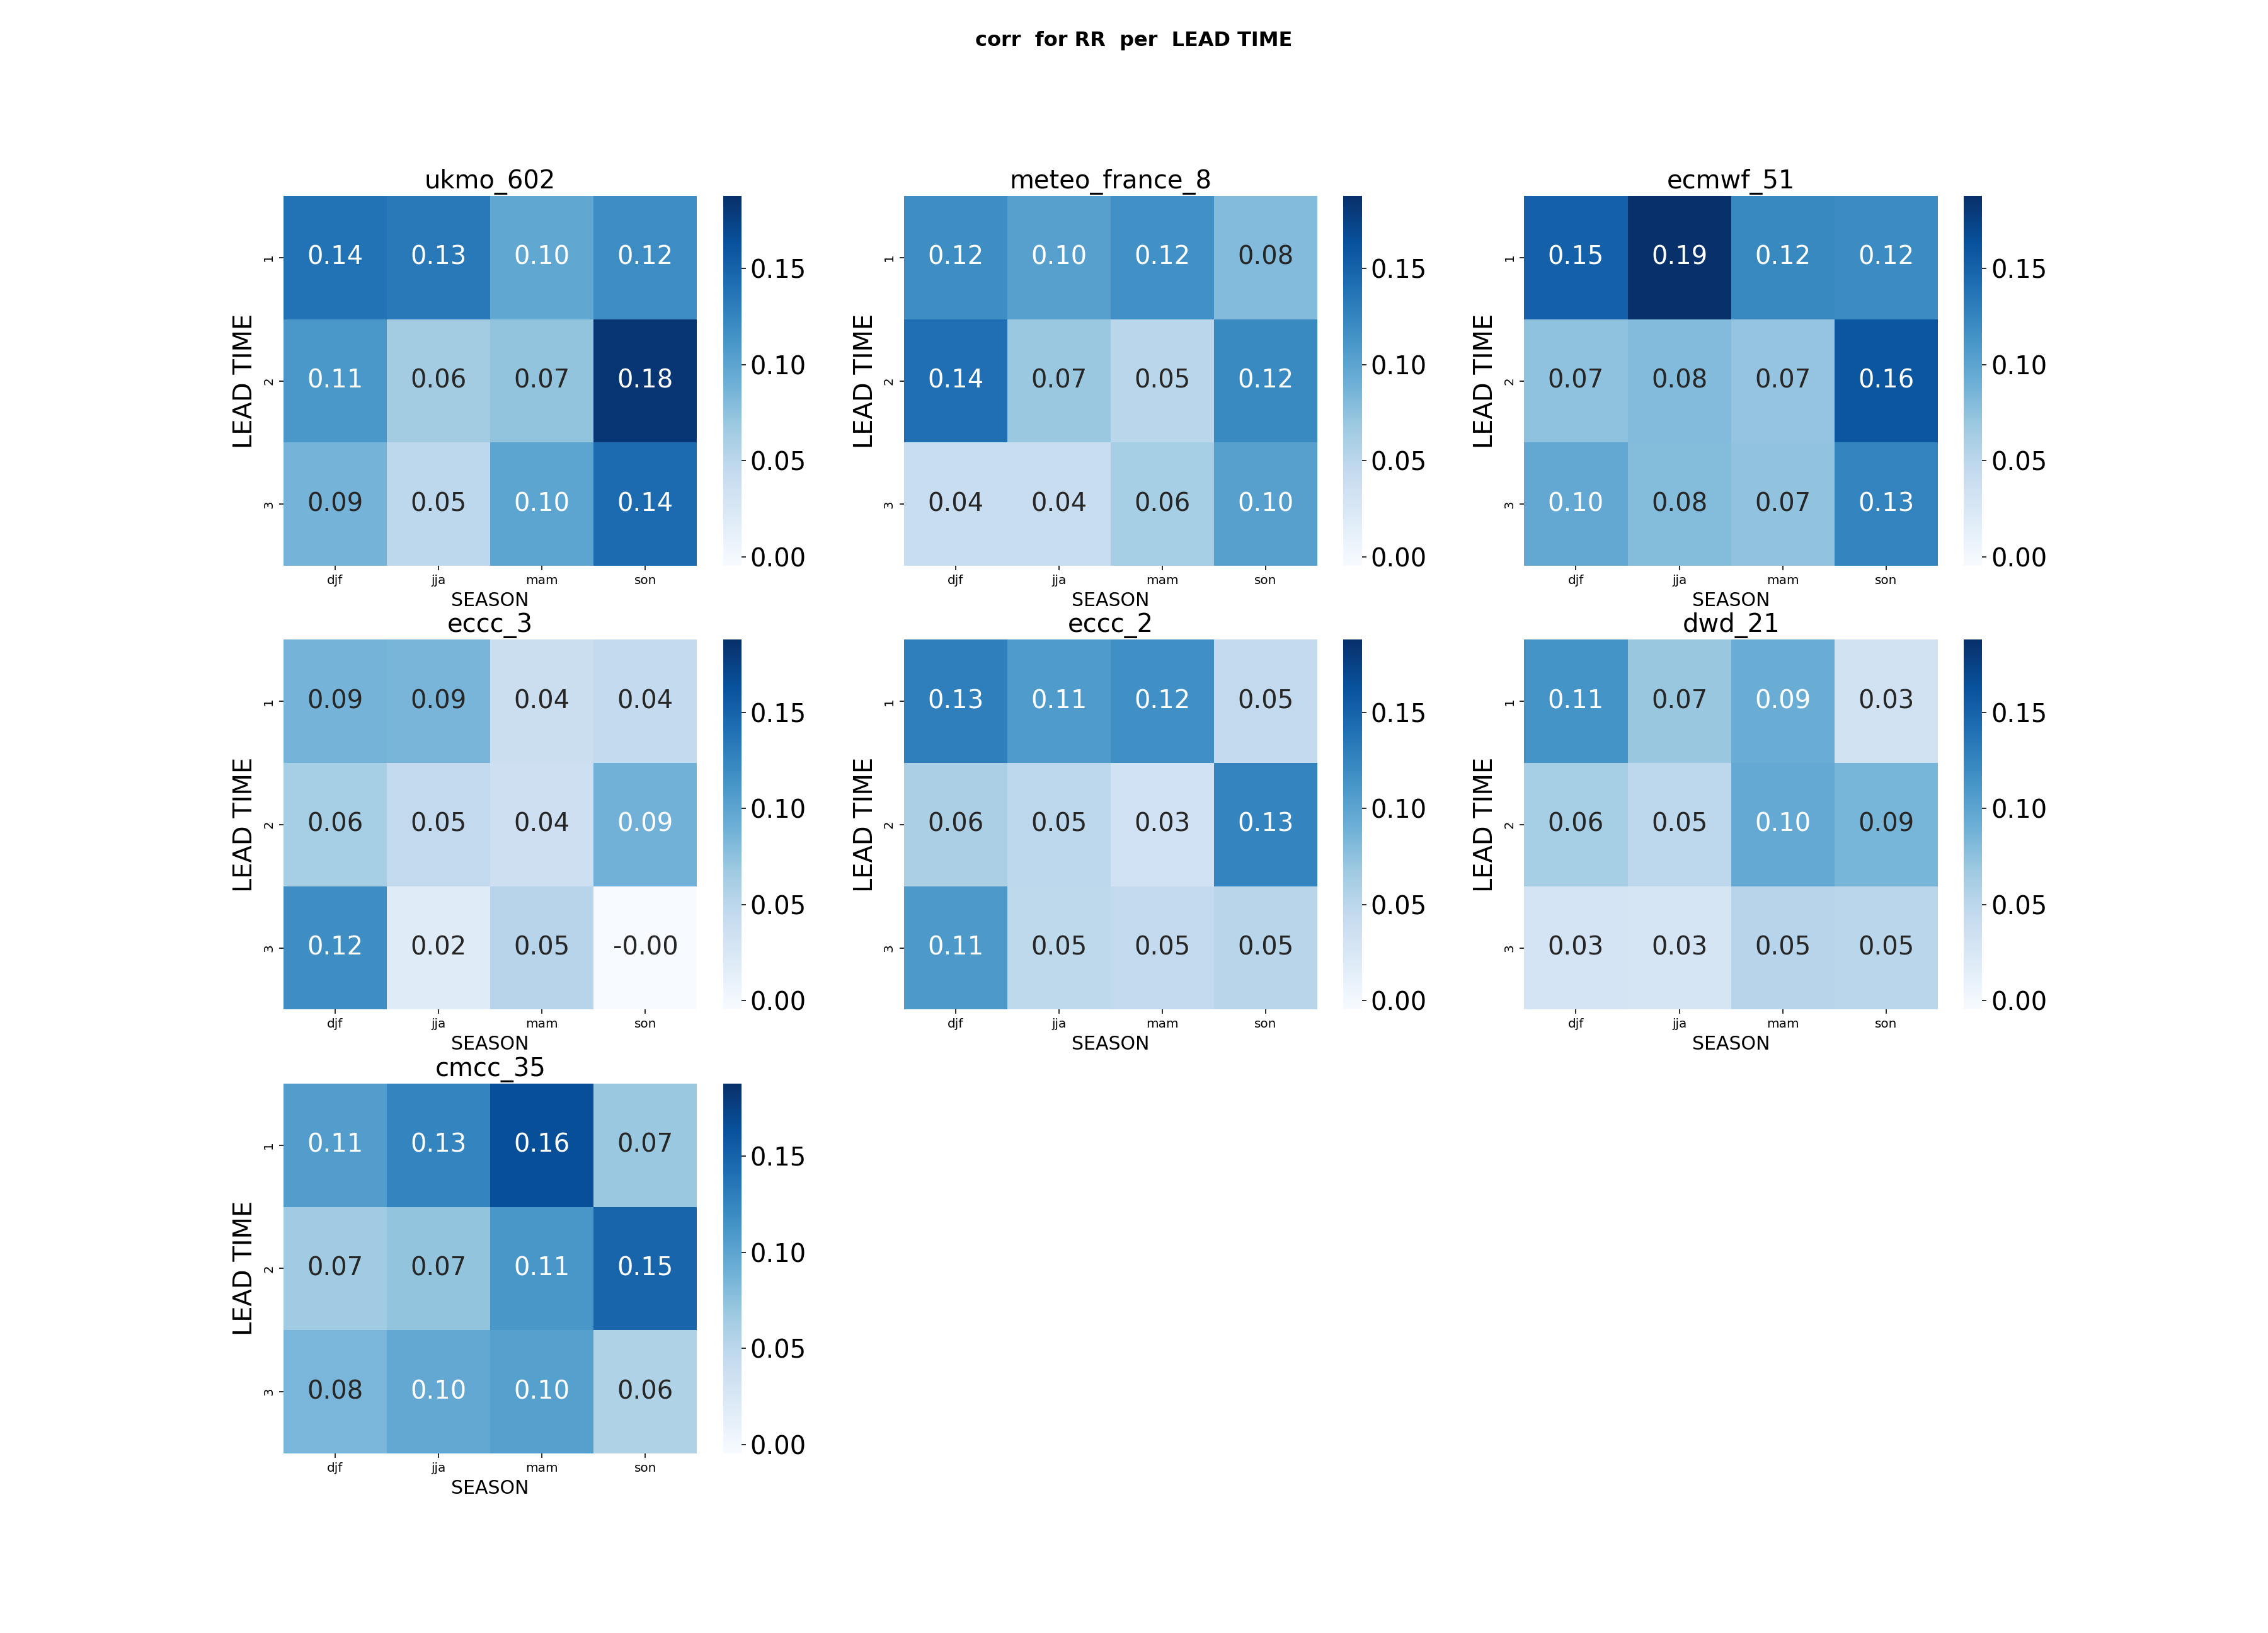
\includegraphics[scale=0.25]{plots/det/corr/corr_RR.png}
	\caption{The Heatmap of correlation for the mena region for every period \textbf{\textit{(1 for perfect Correlation)} }}
\end{figure}
In general, correlation is very week for all centers, the maximum correlation is 0.175 for ecmwf. There is also some differences between centers. We can sea that in general the performance decrease with lead-time. the best models in term of Correlation are \textbf{\textit{ecmwf , ukmo and meteo-france}} .In general the performance decreases with time for all periods except for the SON period where the performance may increase with lead-time. 



\begin{figure}[H]
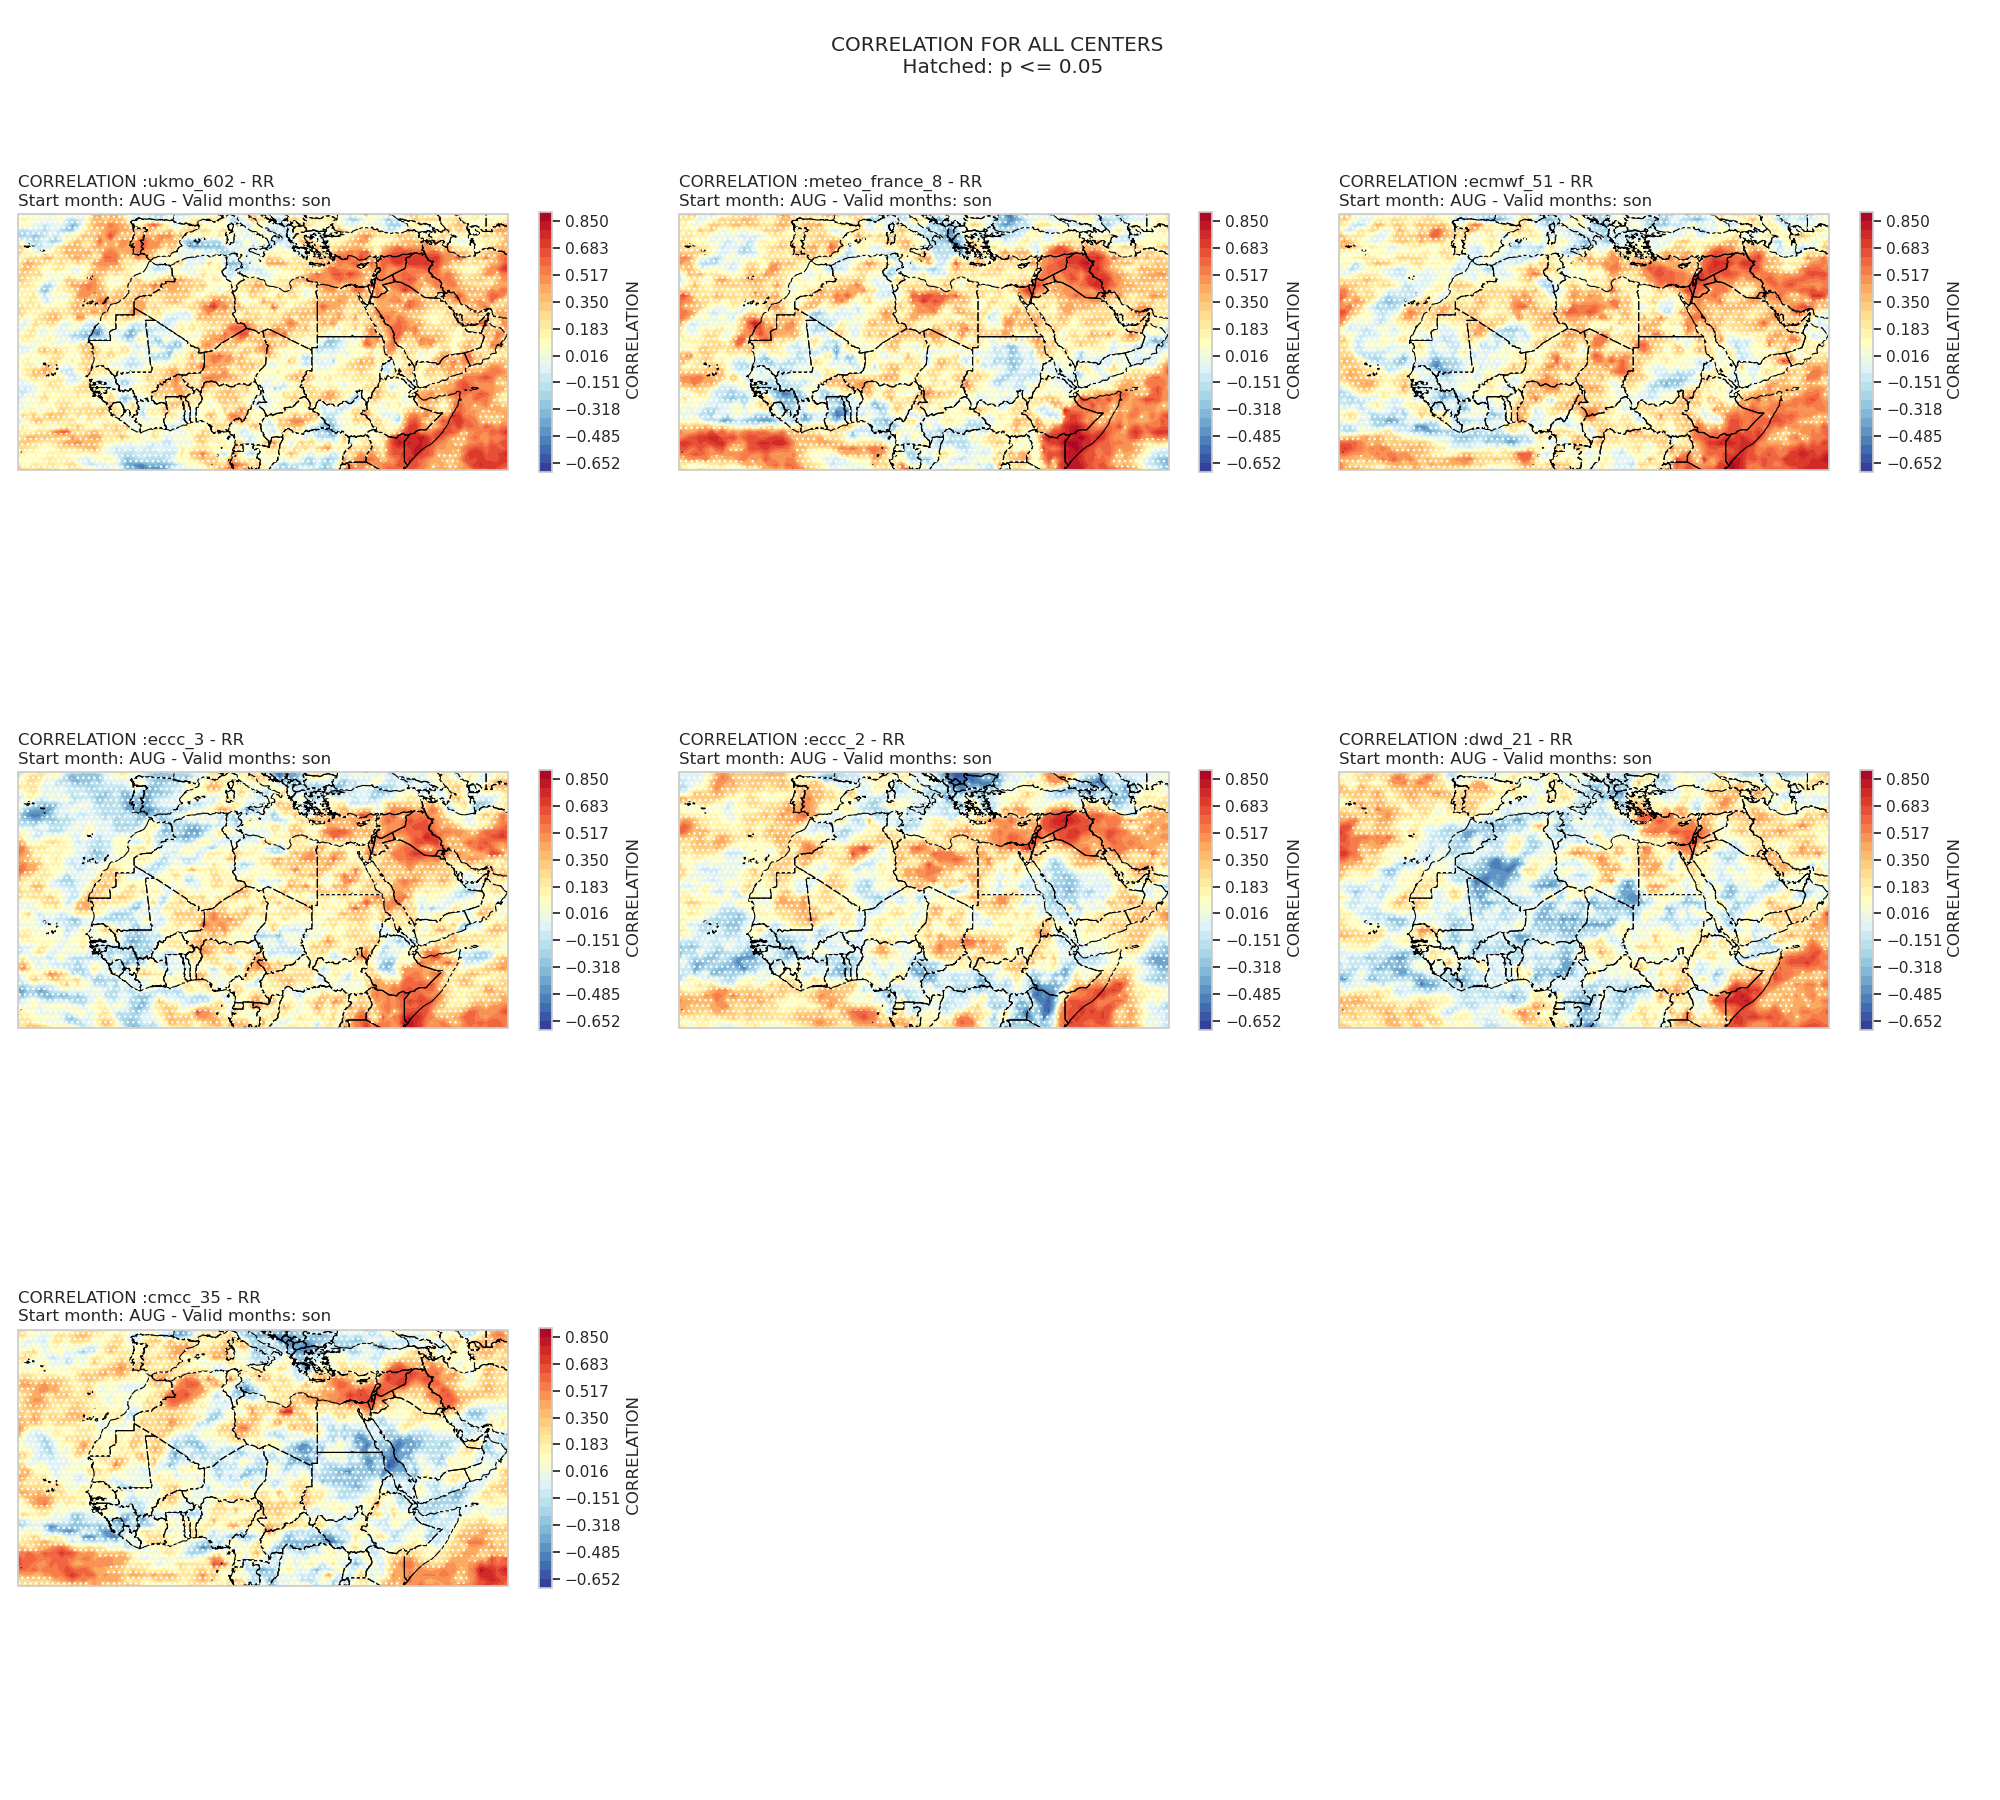
\includegraphics[scale=0.3]{plots/det/corr/CORR_son_RR.png}
\caption{3-months Rolling mean of Spearman Correlation in MENA Region for all centers DJF}
\end{figure}

For temperature, the models demonstrate the best performance in the tropical regions. However, for precipitation, the situation is different. In the figure above, we observe an unusual performance during SON, where the Middle East, East Africa, and North Africa exhibit the highest correlation performance. 


\subsubsection{RMSE}
 
for the Root Mean Squared Error, the best models shown in the heatmap below are \textbf{\textit{DWD, ECMWF and UKMO}}. The RMSE score demonstrate an excellent performance for all models especially \textbf{\textit{DWD, ECMWF and UKMO}}. The performance is stable over lead-times and it is much better for djf in all centers.

\begin{figure}[H]
\includegraphics[scale=0.3]{plots/det/rmse/rmse_RR.png}
\caption{3-months Rolling mean of RMSE in MENA Region for all centers DJF}
\end{figure}

\begin{figure}[H]
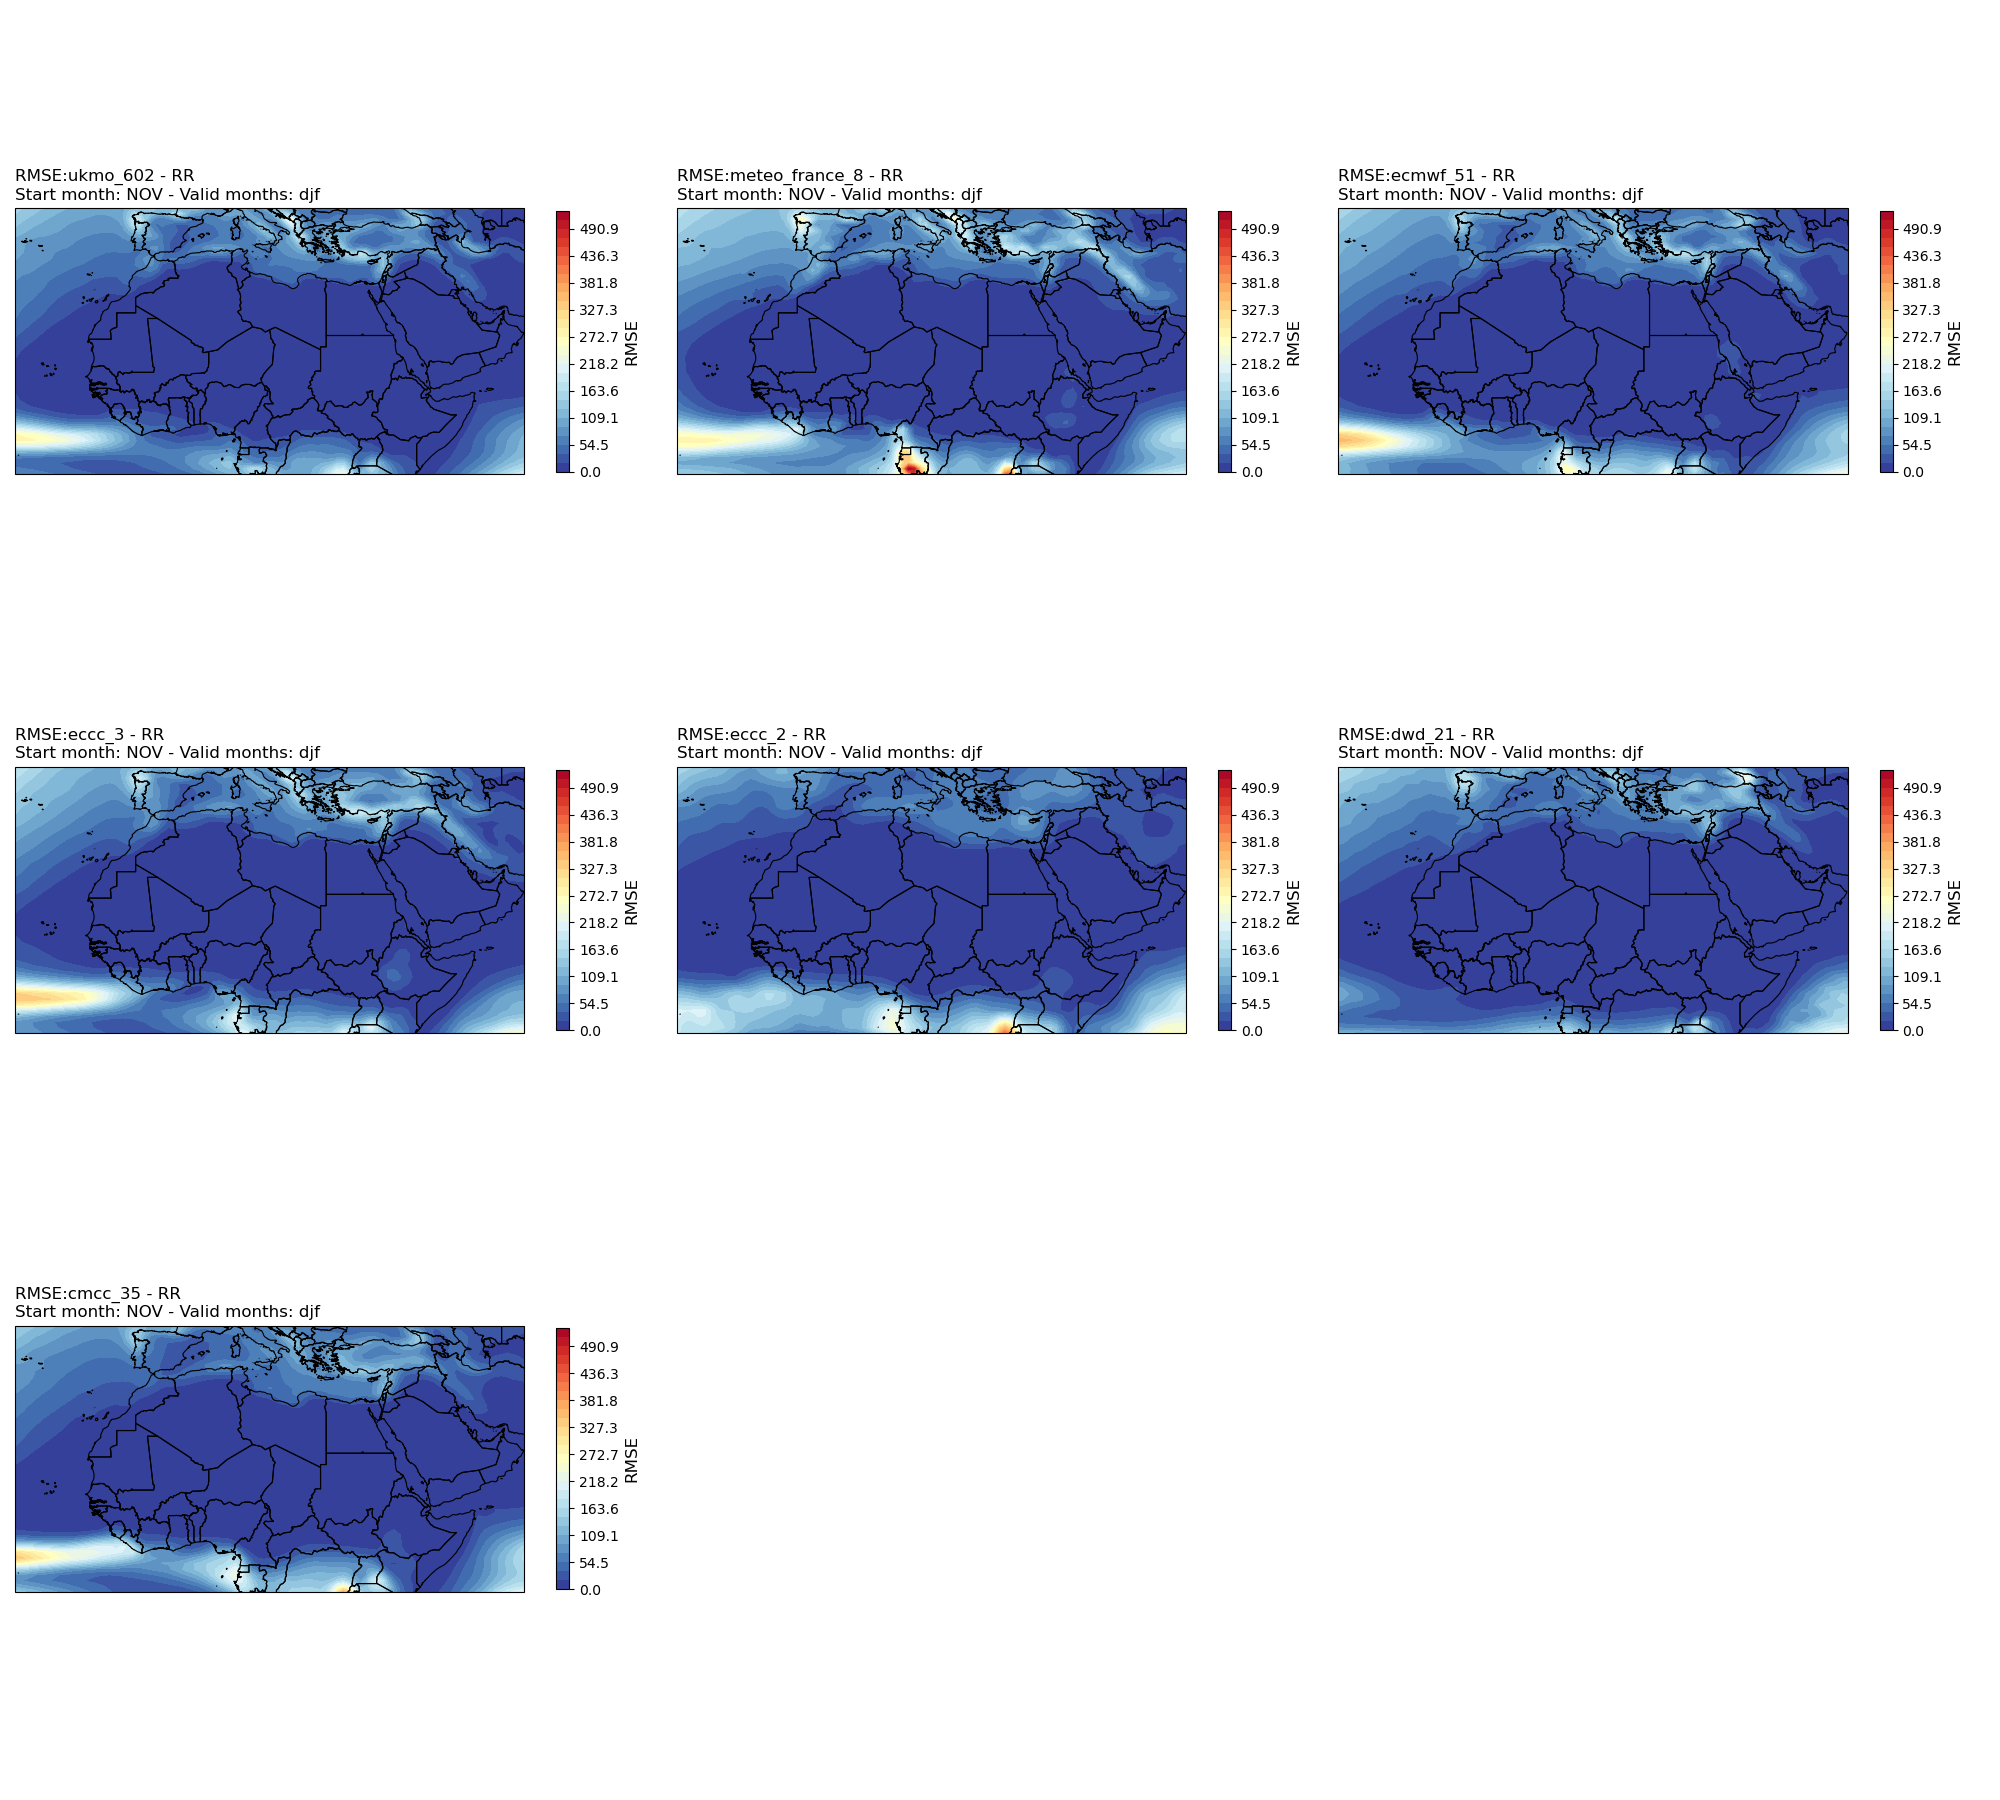
\includegraphics[scale=0.3]{plots/det/rmse/rmse_djf_RR.png}
\caption{3-months Rolling mean of RMSE in MENA Region for all centers JJA}
\end{figure}

also for the spacial dimension, the RMSE stay stable and exhibit very good performance for all centers. 


\subsubsection{Coefficient of Determination (\( R^2 \))}

for precipitation, the R-SQUARED is very low, the maximum value is less than 0.1. However, the ecmwf is the best in term of R-SQUARED.
\begin{figure}[H]
	\centering
	\includegraphics[scale=0.25]{plots/det/rsquared/rsquared_RR.png}
	\caption{The Heatmap of rsquared for Precipitations in the mena region for every period \textbf{\textit{(1 for perfect RSQUARED)} }}
\end{figure}



\begin{figure}[H]
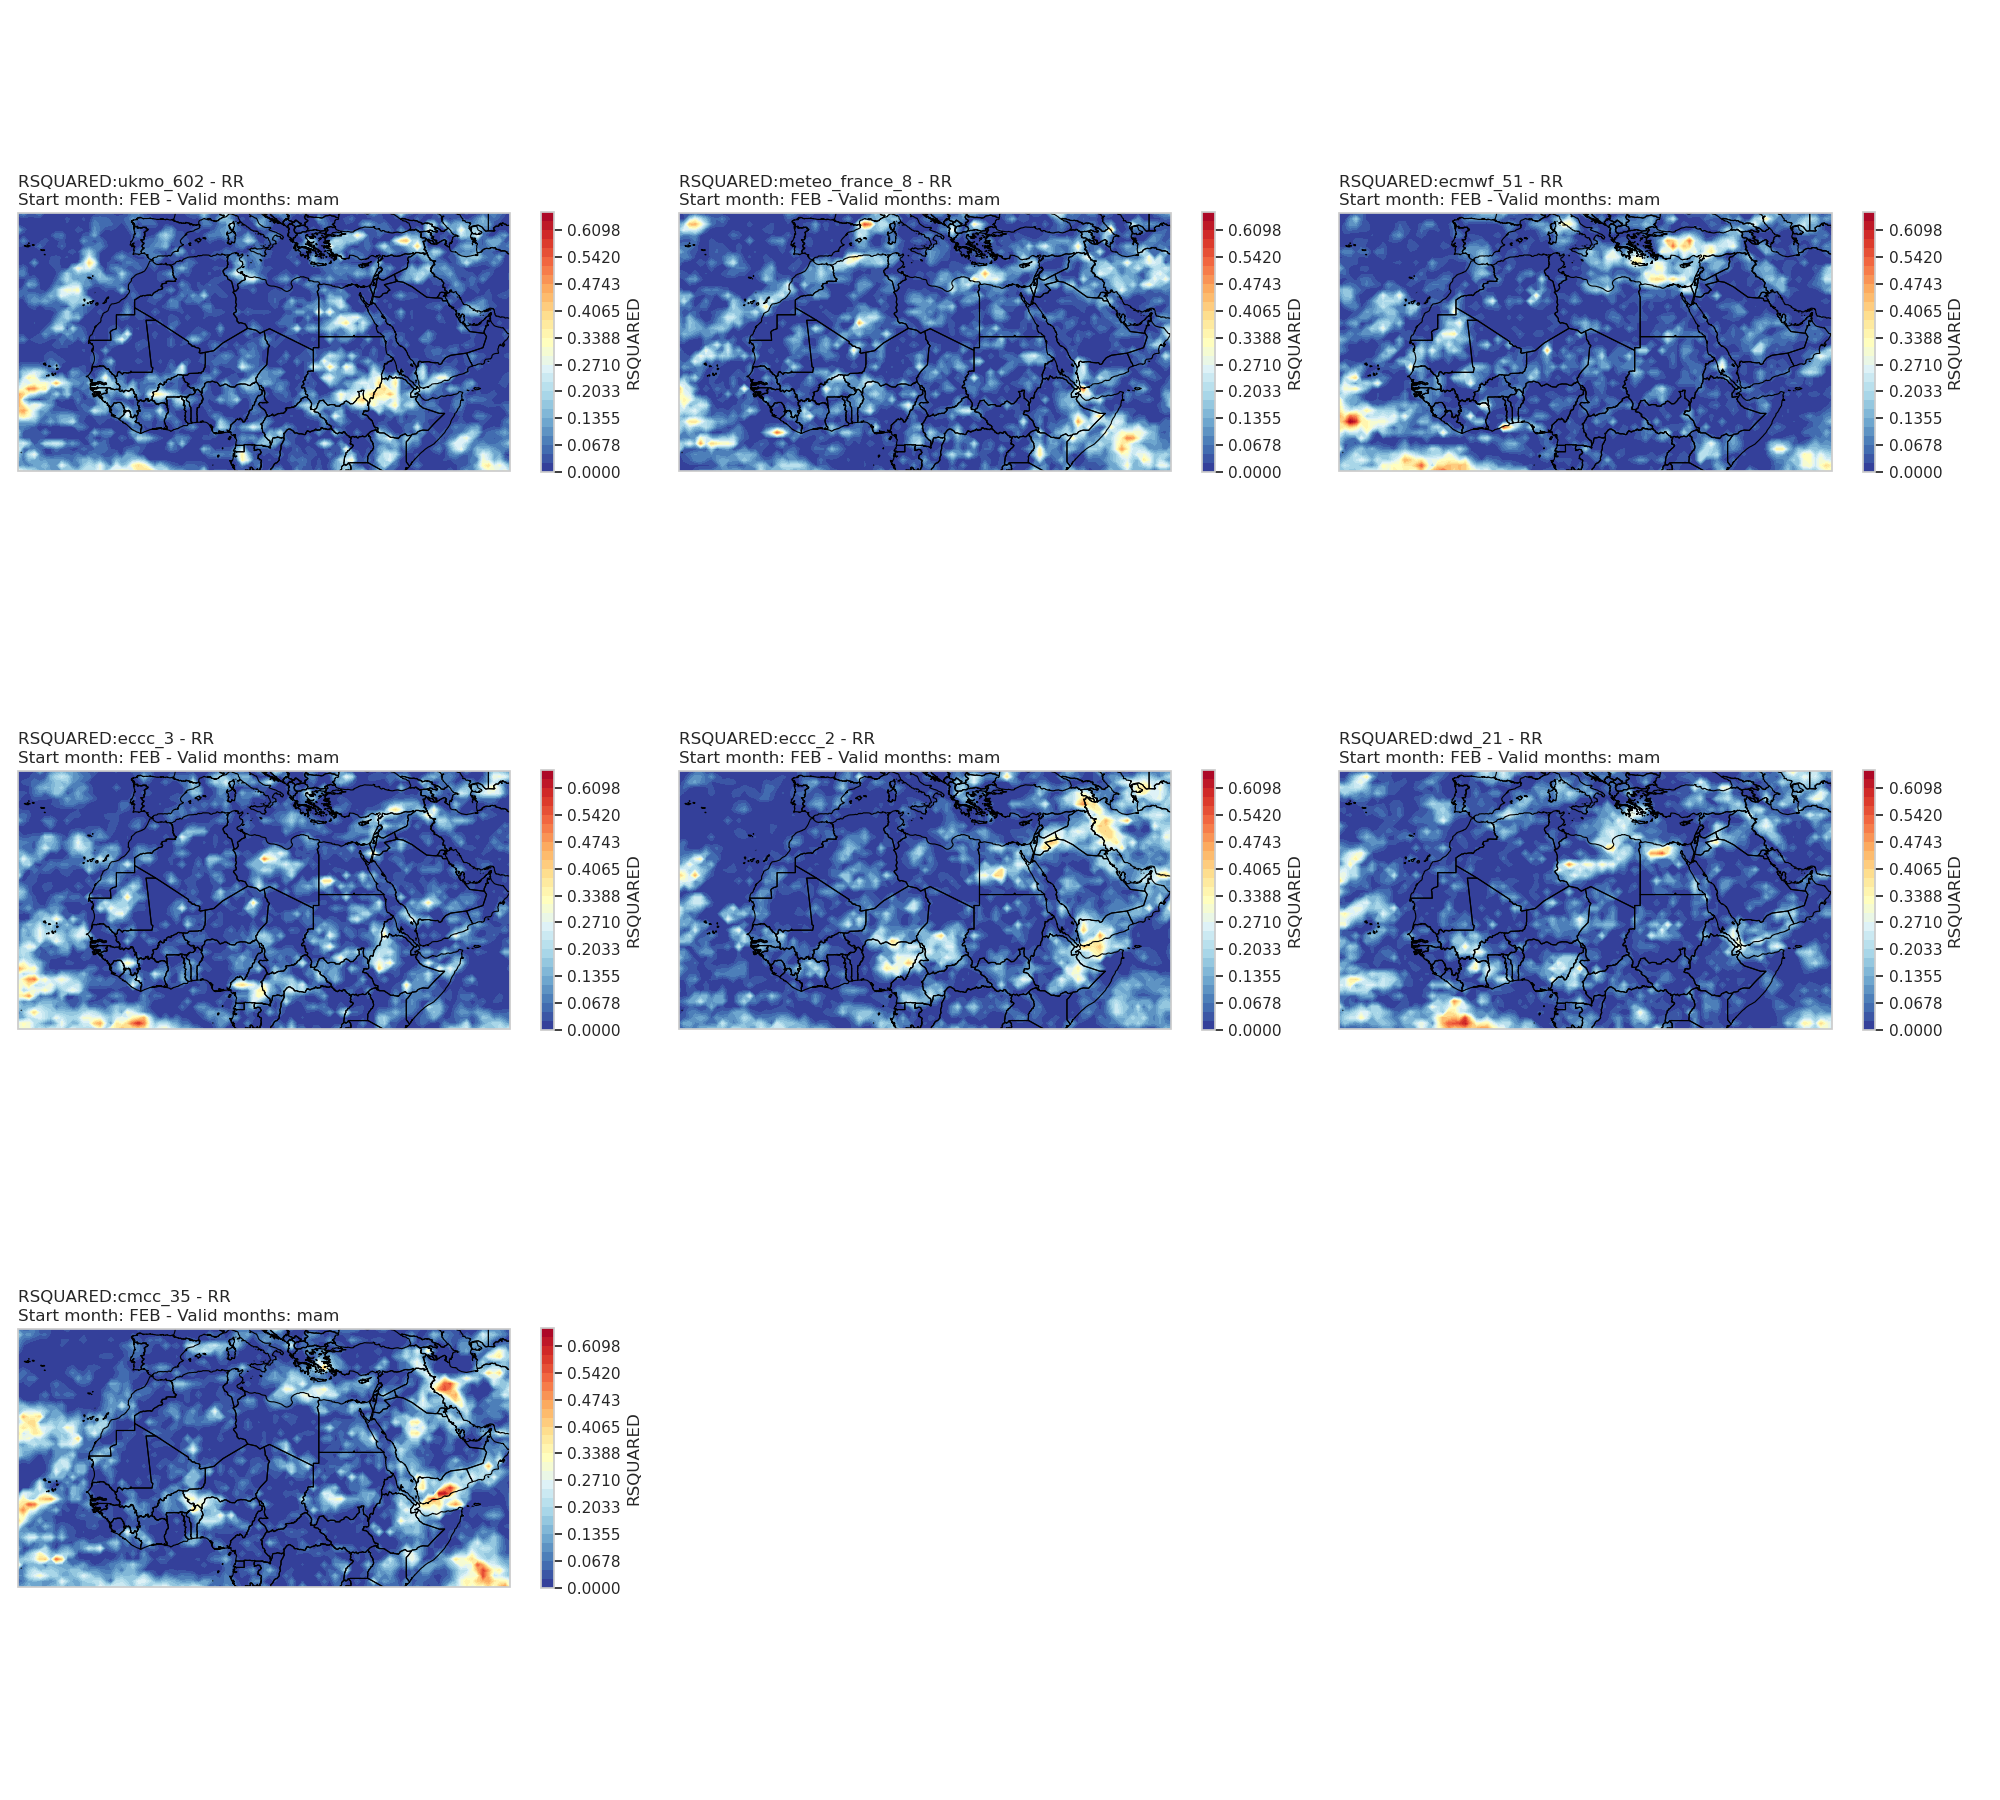
\includegraphics[scale=0.3]{plots/det/rsquared/rsquared_mam_RR.png}
\caption{3-months Rolling mean of RSQUARED in MENA Region for all centers MAM}
\end{figure}

there is some isolated zones where the rsquared is good especially in the Middle East for CMCC-35 Center or the equator for DWD, but in general the score is very low.


\subsection{Probabilistic Evaluation Metrics}

\subsubsection{The Brier Score (BS)}

\begin{figure}[H]
    \centering
    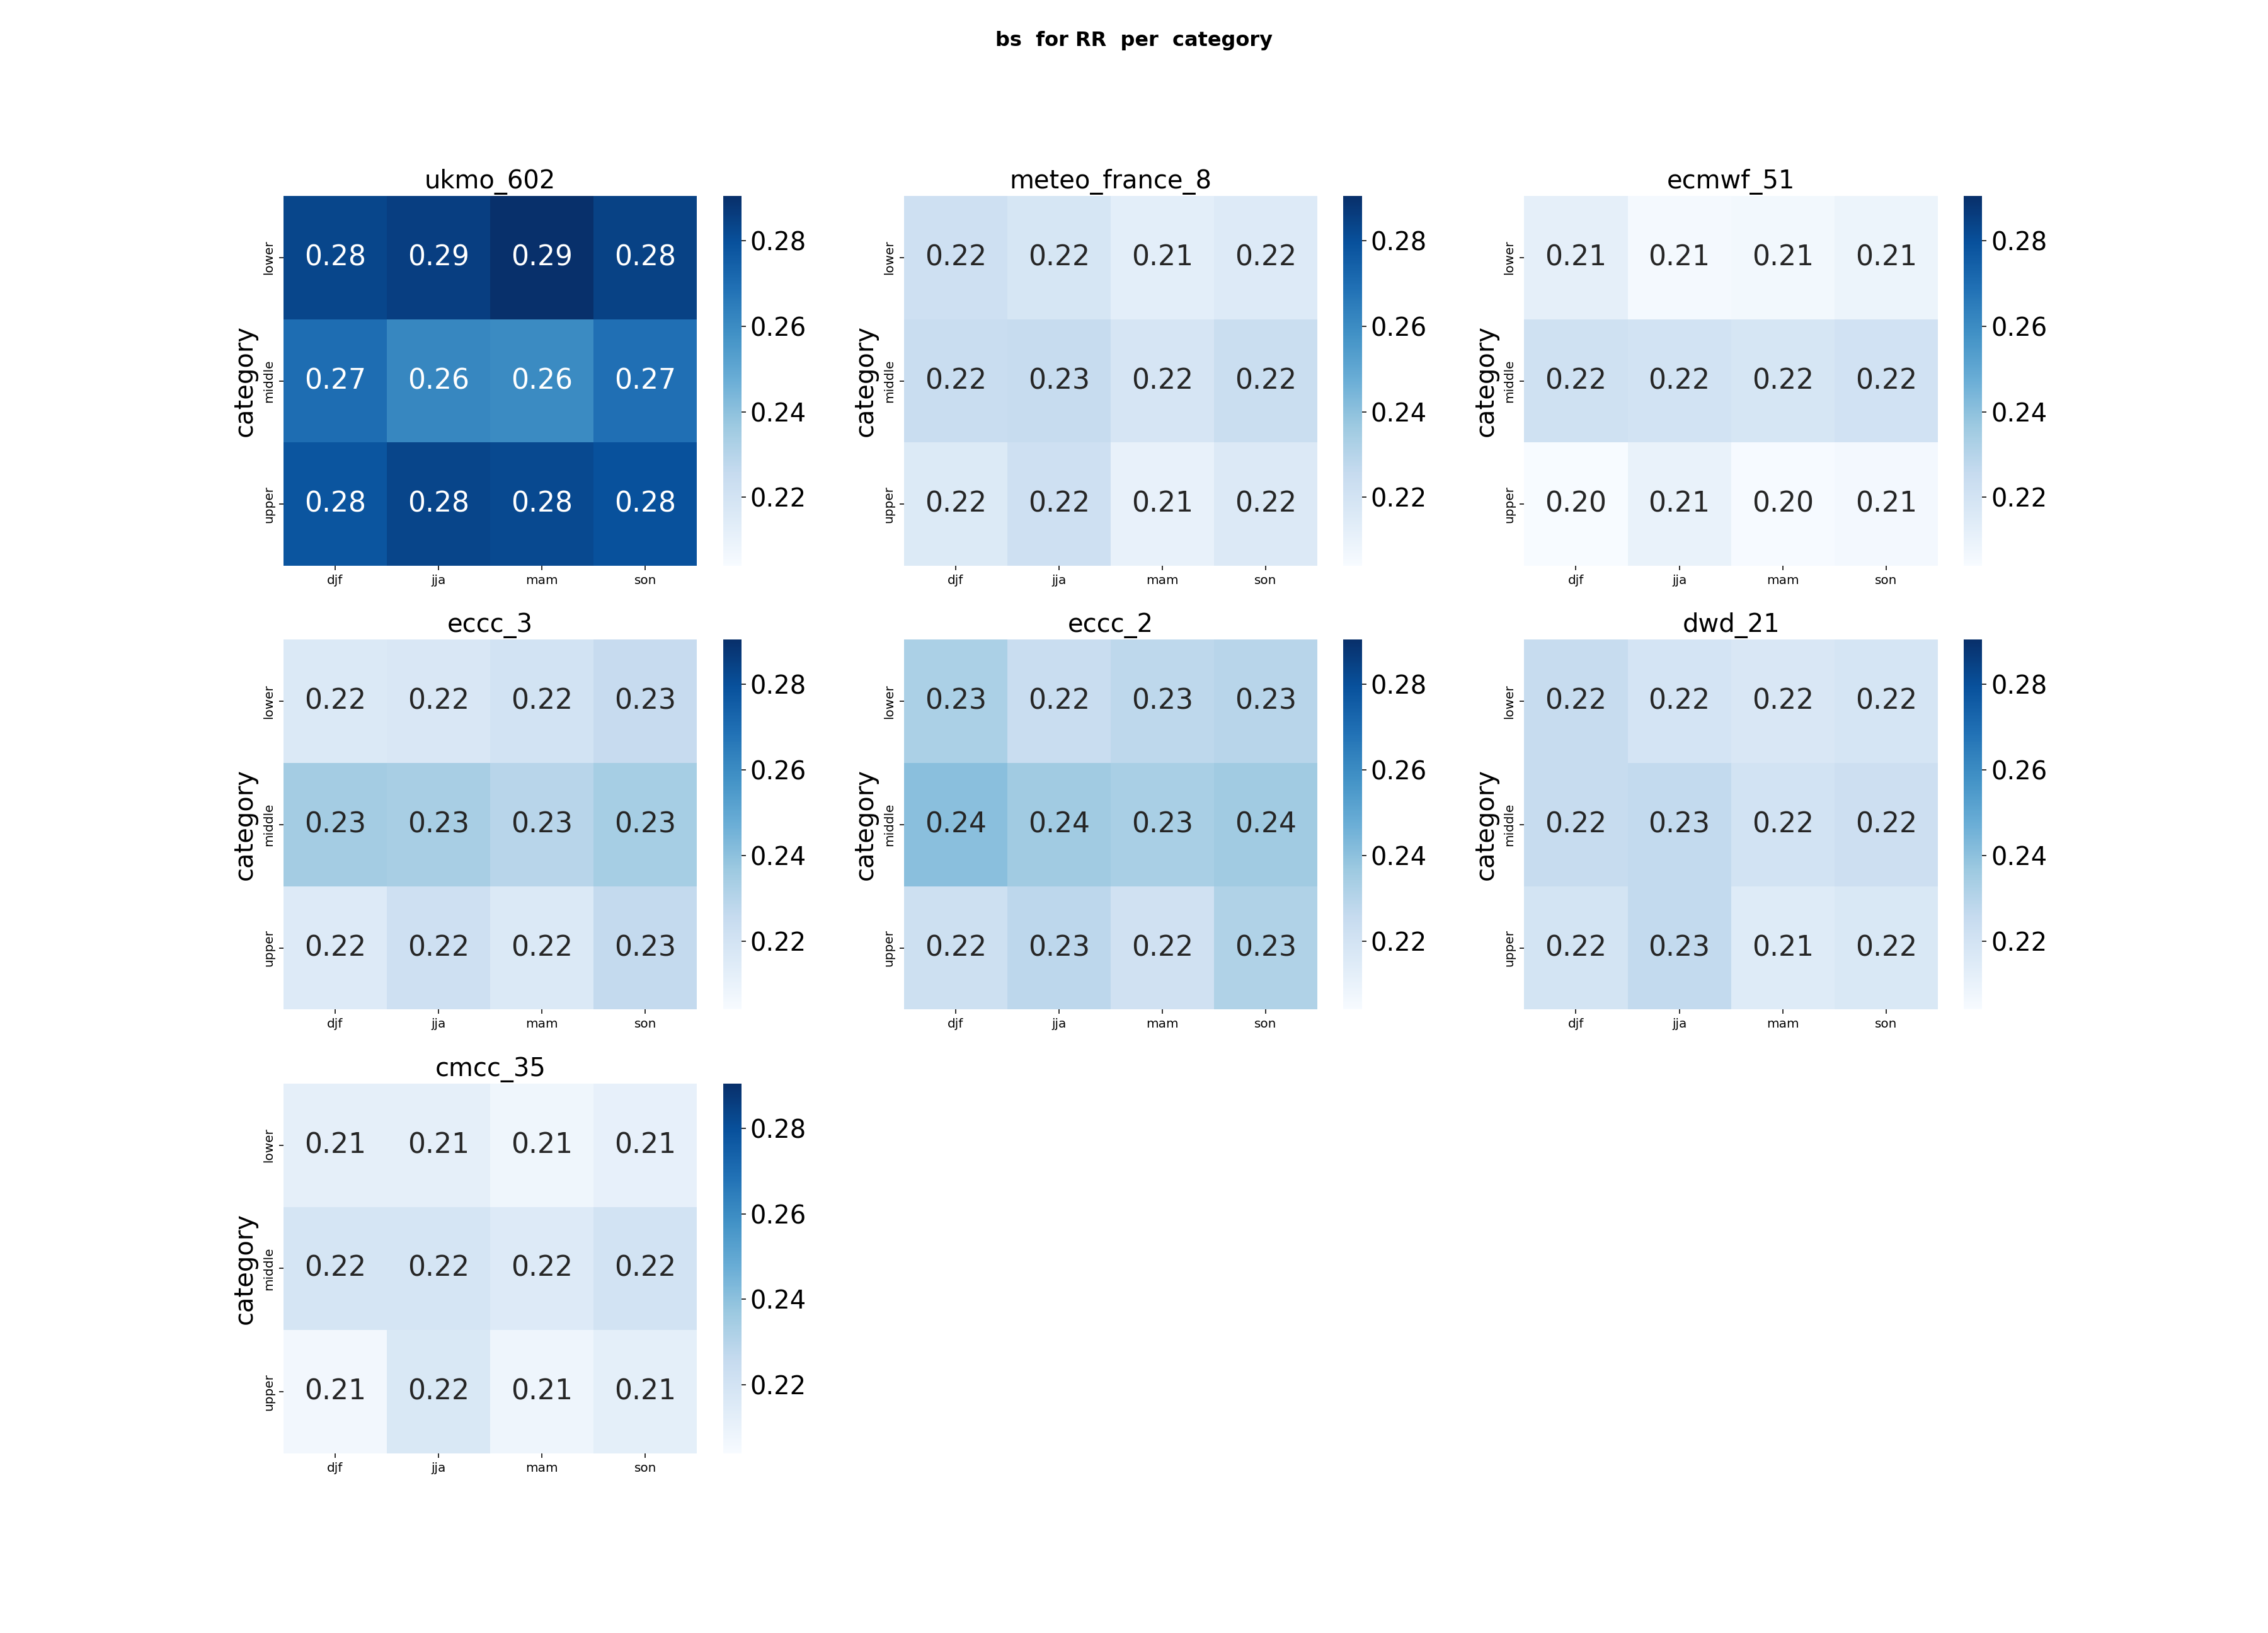
\includegraphics[scale=0.25]{plots/prob/bs/bs_RR_category.png}
    \caption{The Heatmap of Brier Score for each category  . \textbf{\textit{(0 represents perfect BS)}}}
\end{figure}

for the analysis per category, we can see in the figure above that all centers exhibit good performance in term of Brier Score except the UMKO that shows moderate BS.
the figure below shows the analysis per lead-time. the same result is found, but the \textbf{\textit{ECMWF,METEO-FRANCE and CMCC-35}} are the best models in Brier Score for lead-time analysis. \\ 
In general, the performance stays stable over category, lead-time and space.


\begin{figure}[H]
    \centering
    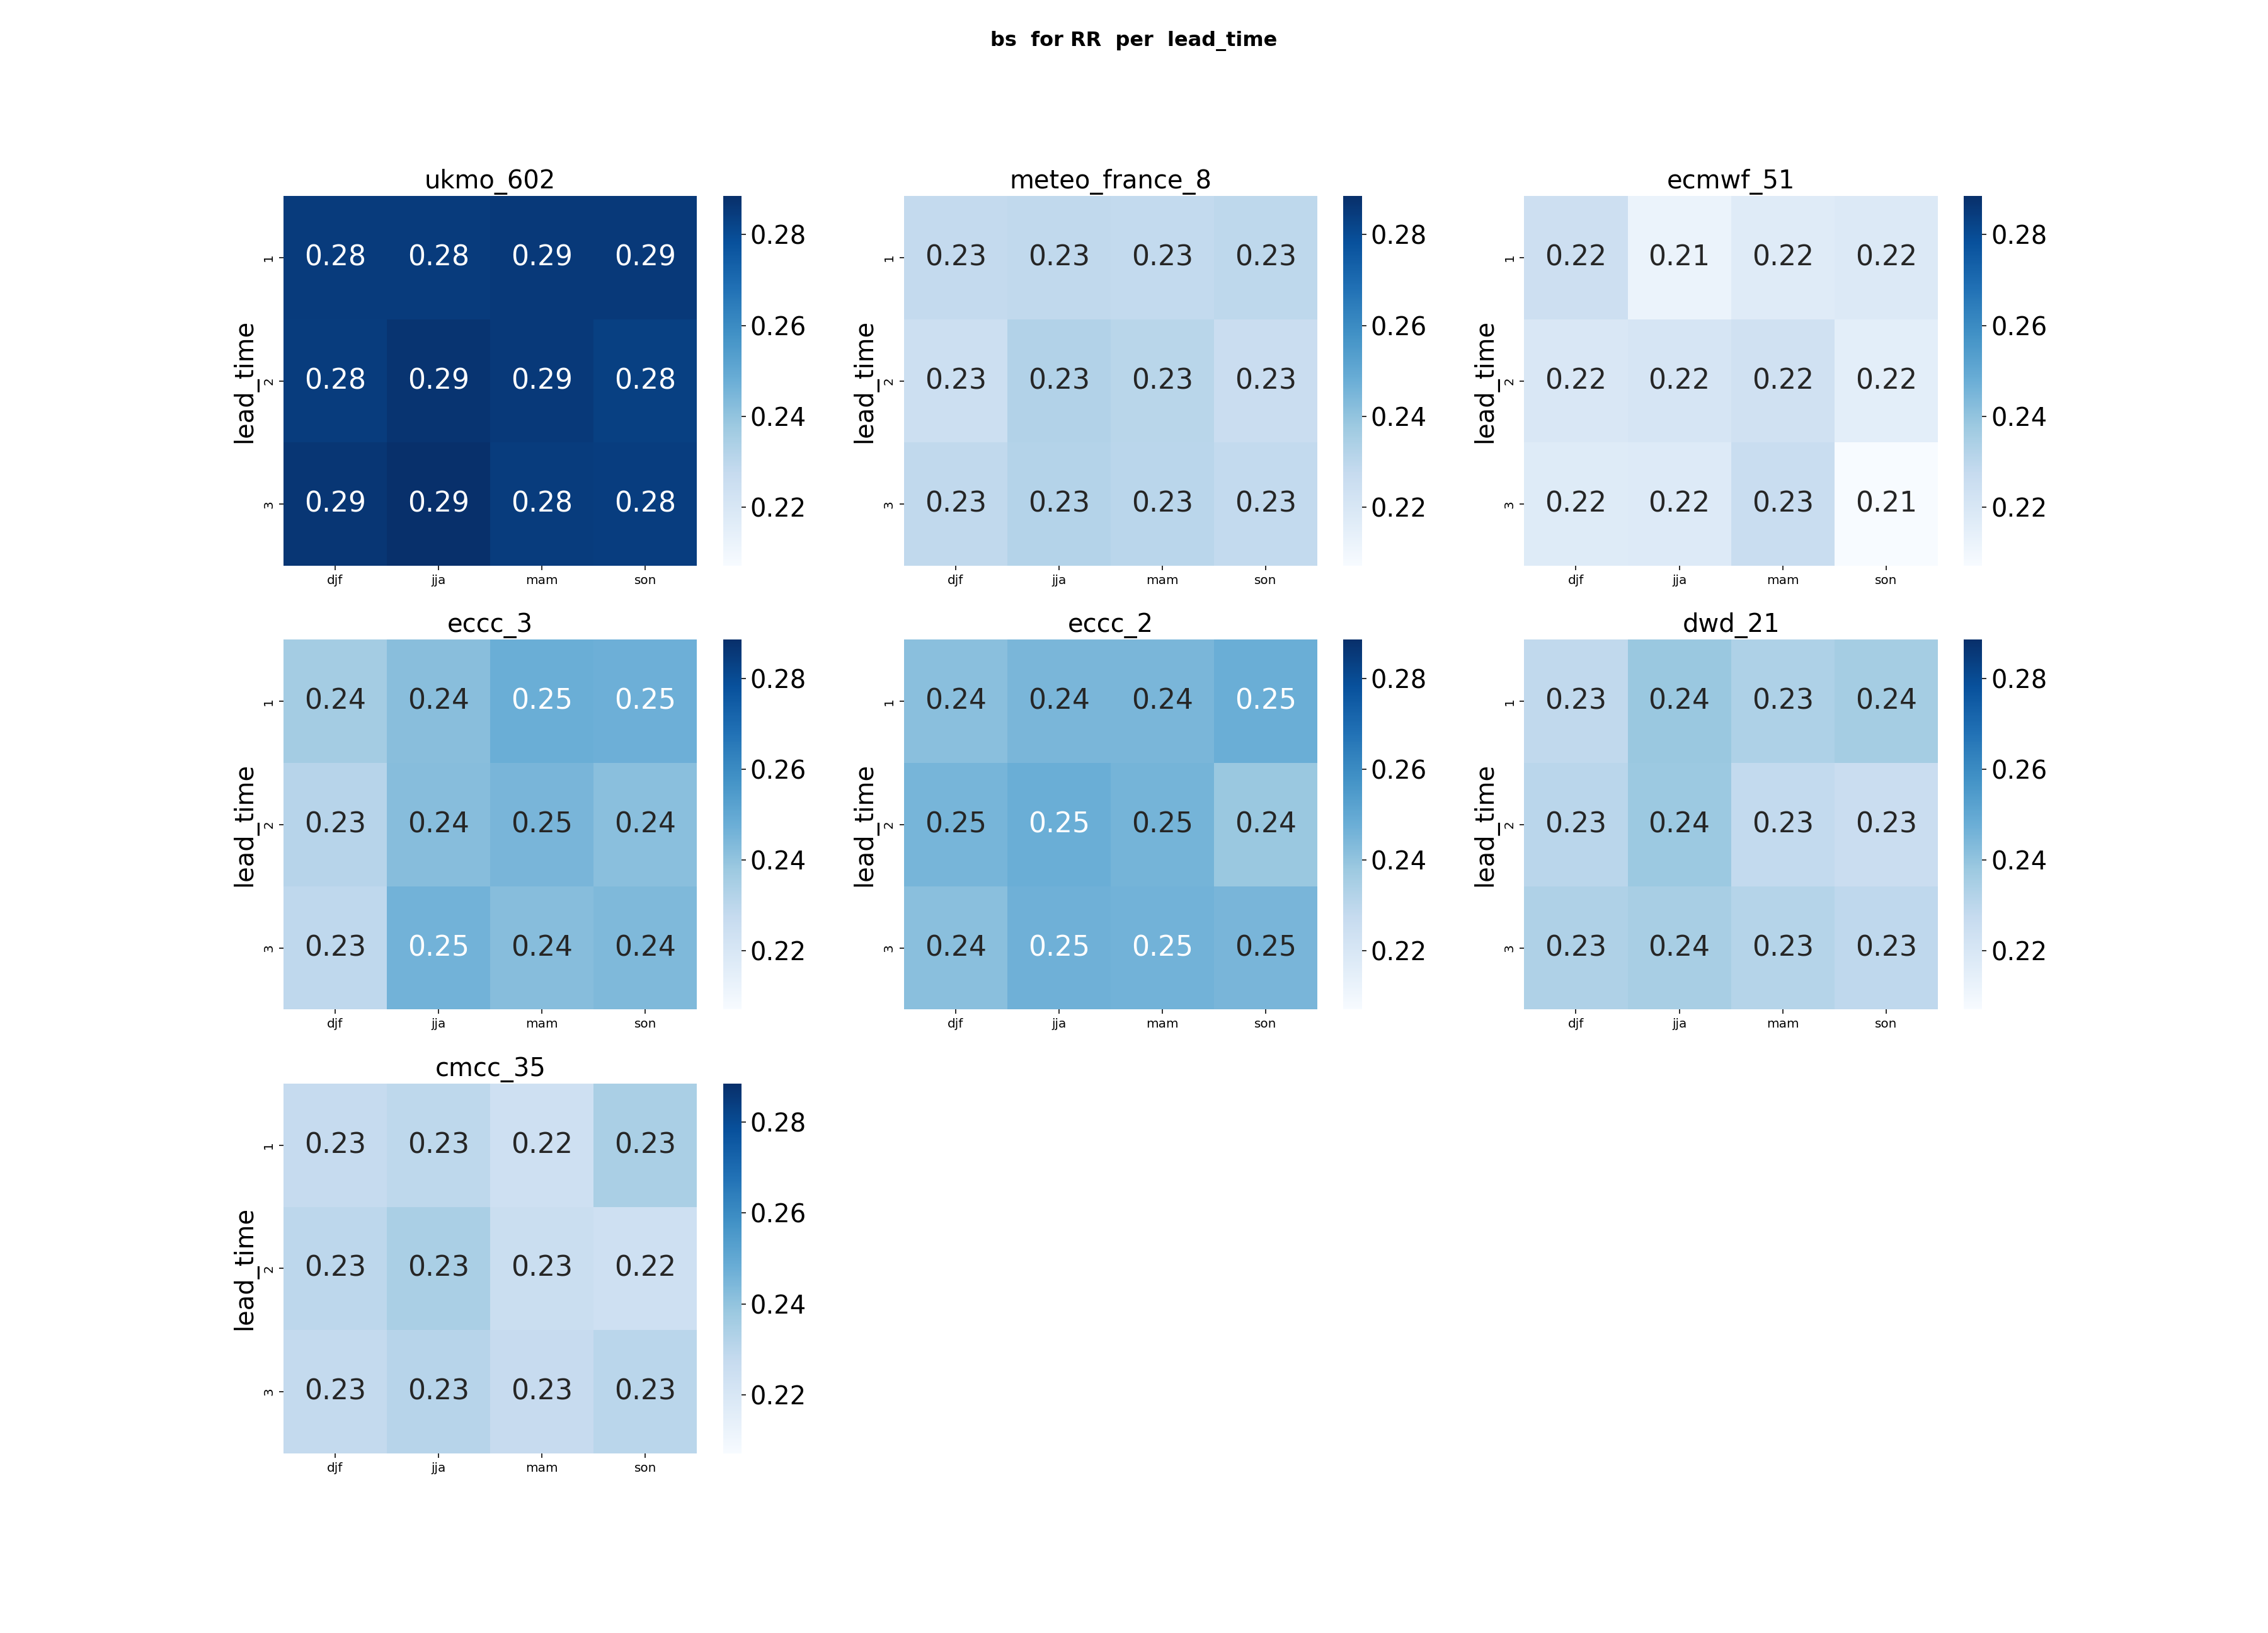
\includegraphics[scale=0.25]{plots/prob/bs/bs_RR_lead_time.png}
    \caption{The Heatmap of Brier Score for lead-time. \textbf{\textit{(0 represents perfect BS)}}}
\end{figure}




\subsubsection{Reliability}

\begin{figure}[H]
    \centering
    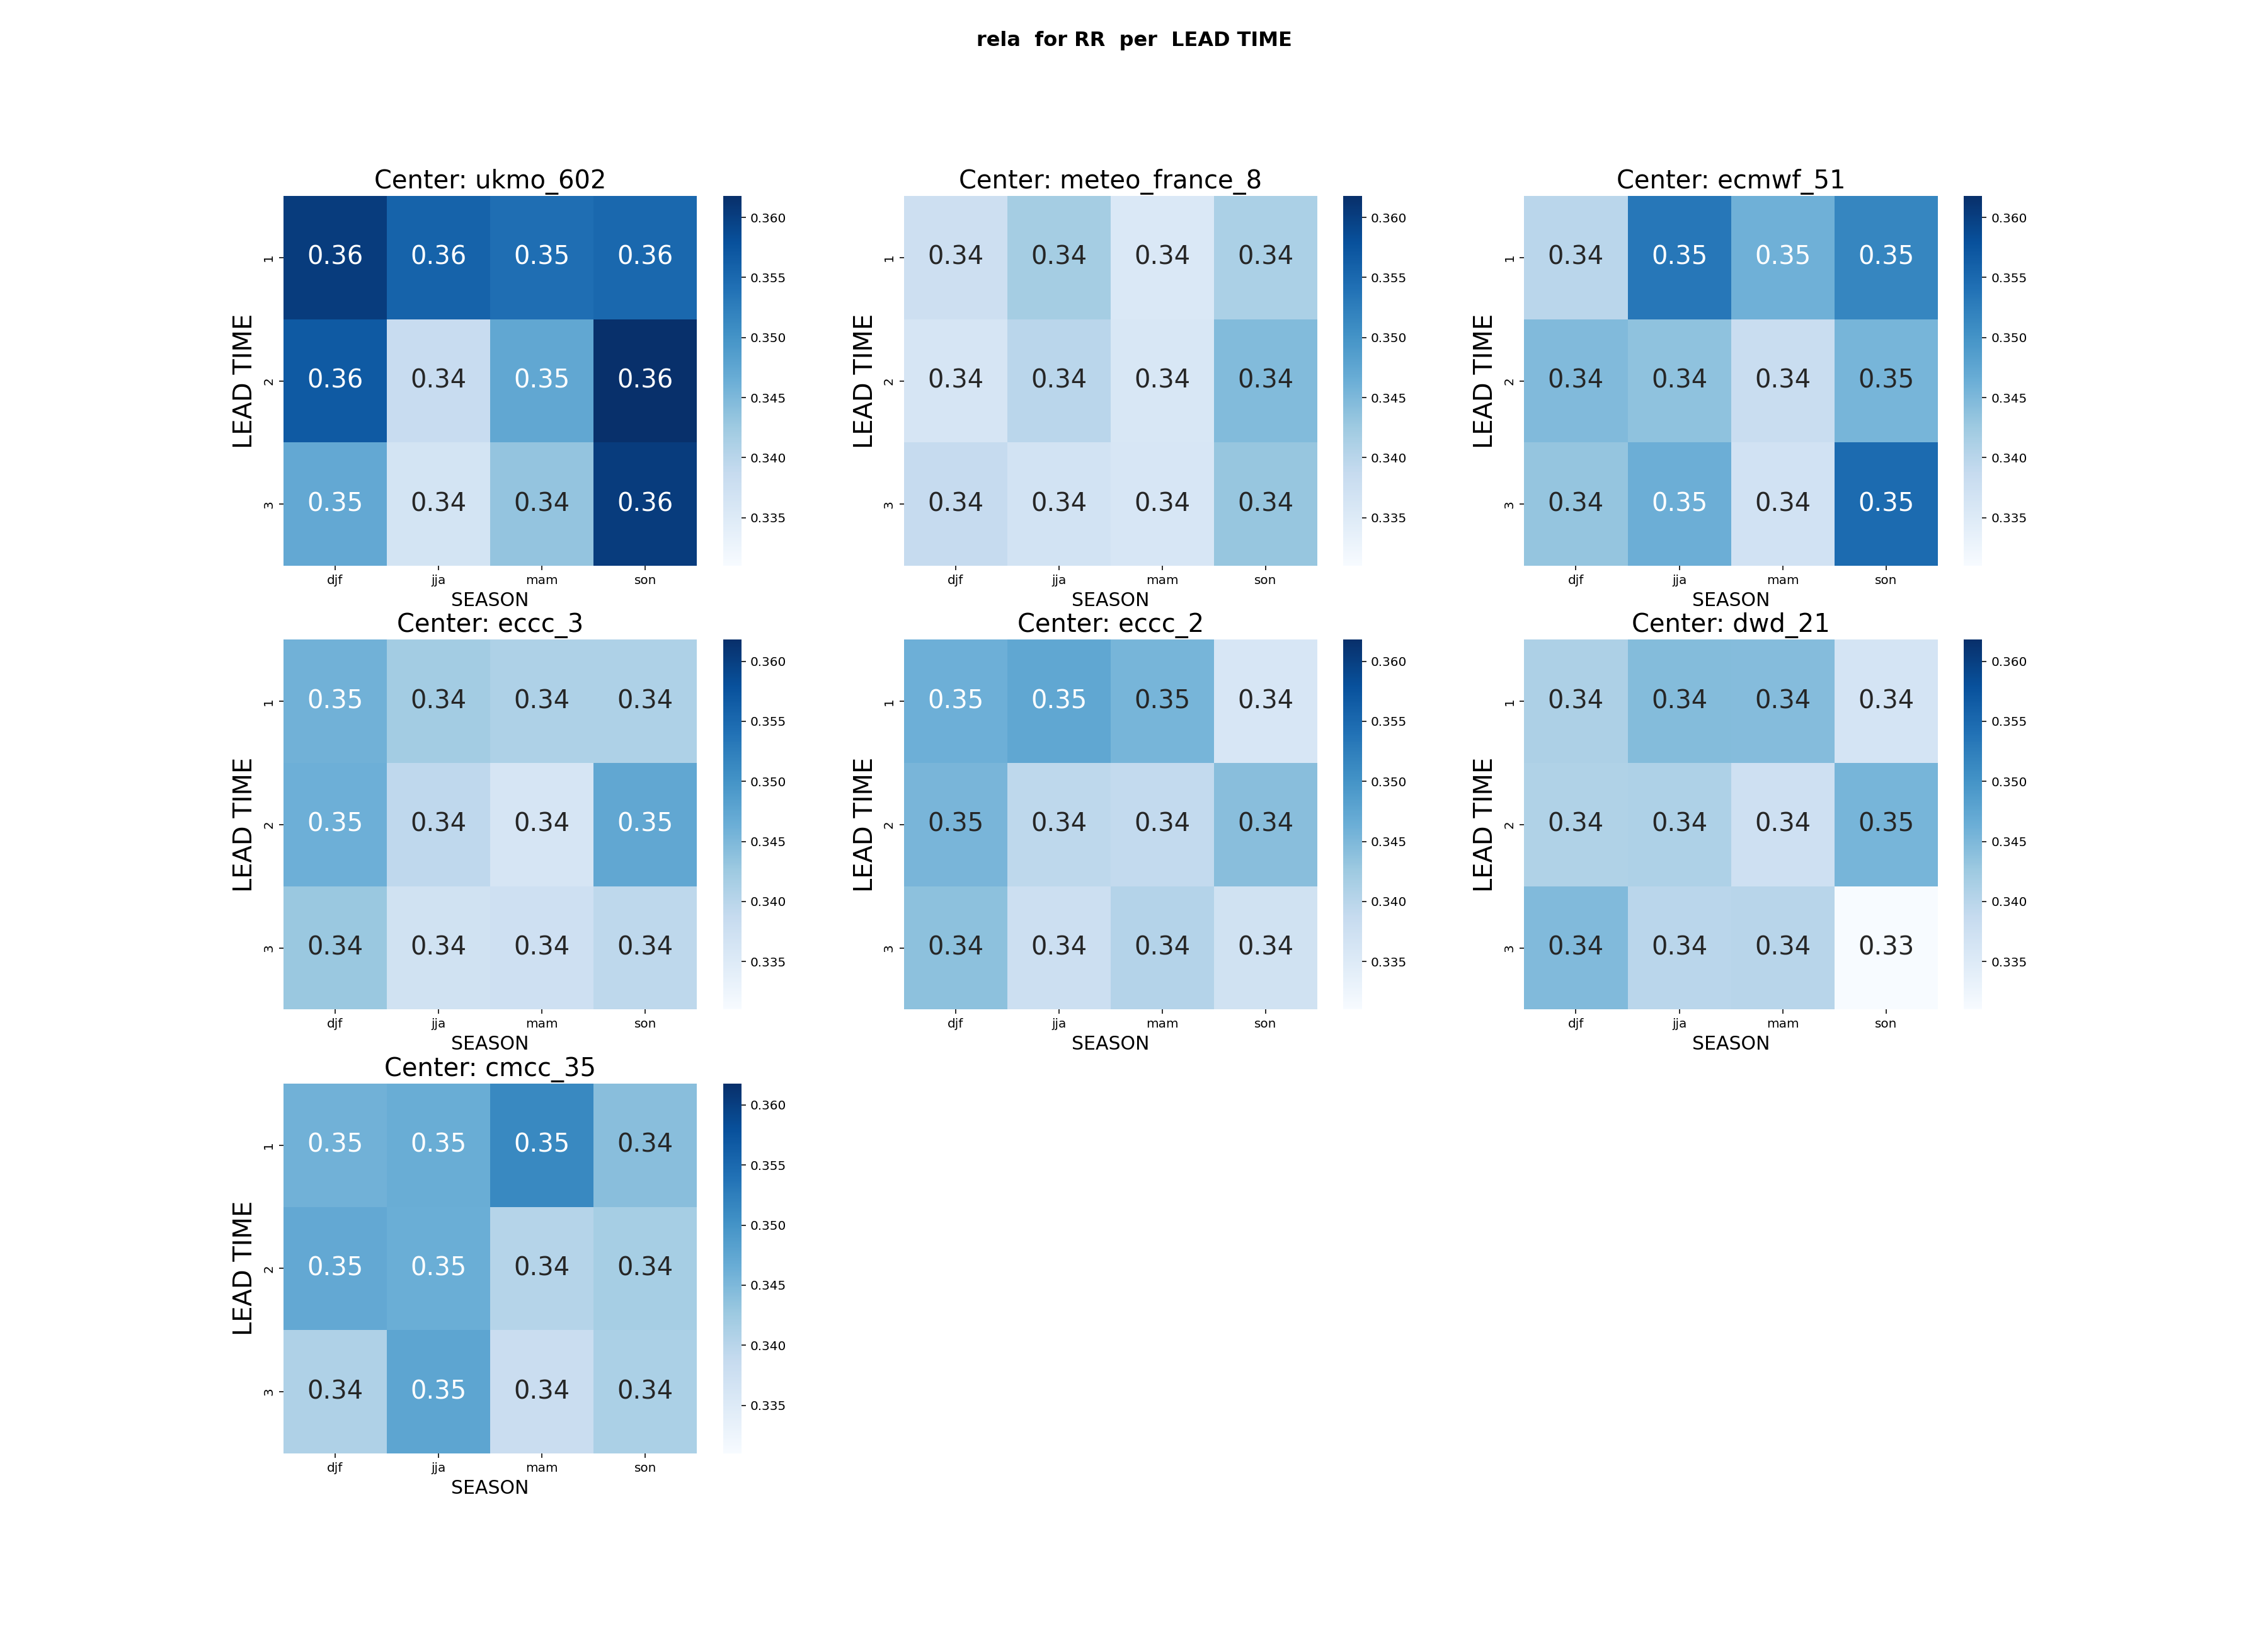
\includegraphics[scale=0.25]{plots/prob/rela/rela_RR.png}
    \caption{The Reliability Score  . \textbf{\textit{(0 means perfect Reliability)}}}
\end{figure}

In the figure above, all centers demonstrate similar moderate performance in term of reliability. But deep analysis within the figure below, shows that UKMO has very bad performance, also we can distinguish three models that have the best reliability according to the reliability diagram, the centers are \textbf{\textit{ECMWF,CMCC and METEO-FRANCE}}. 

\begin{figure}[H]
\centering
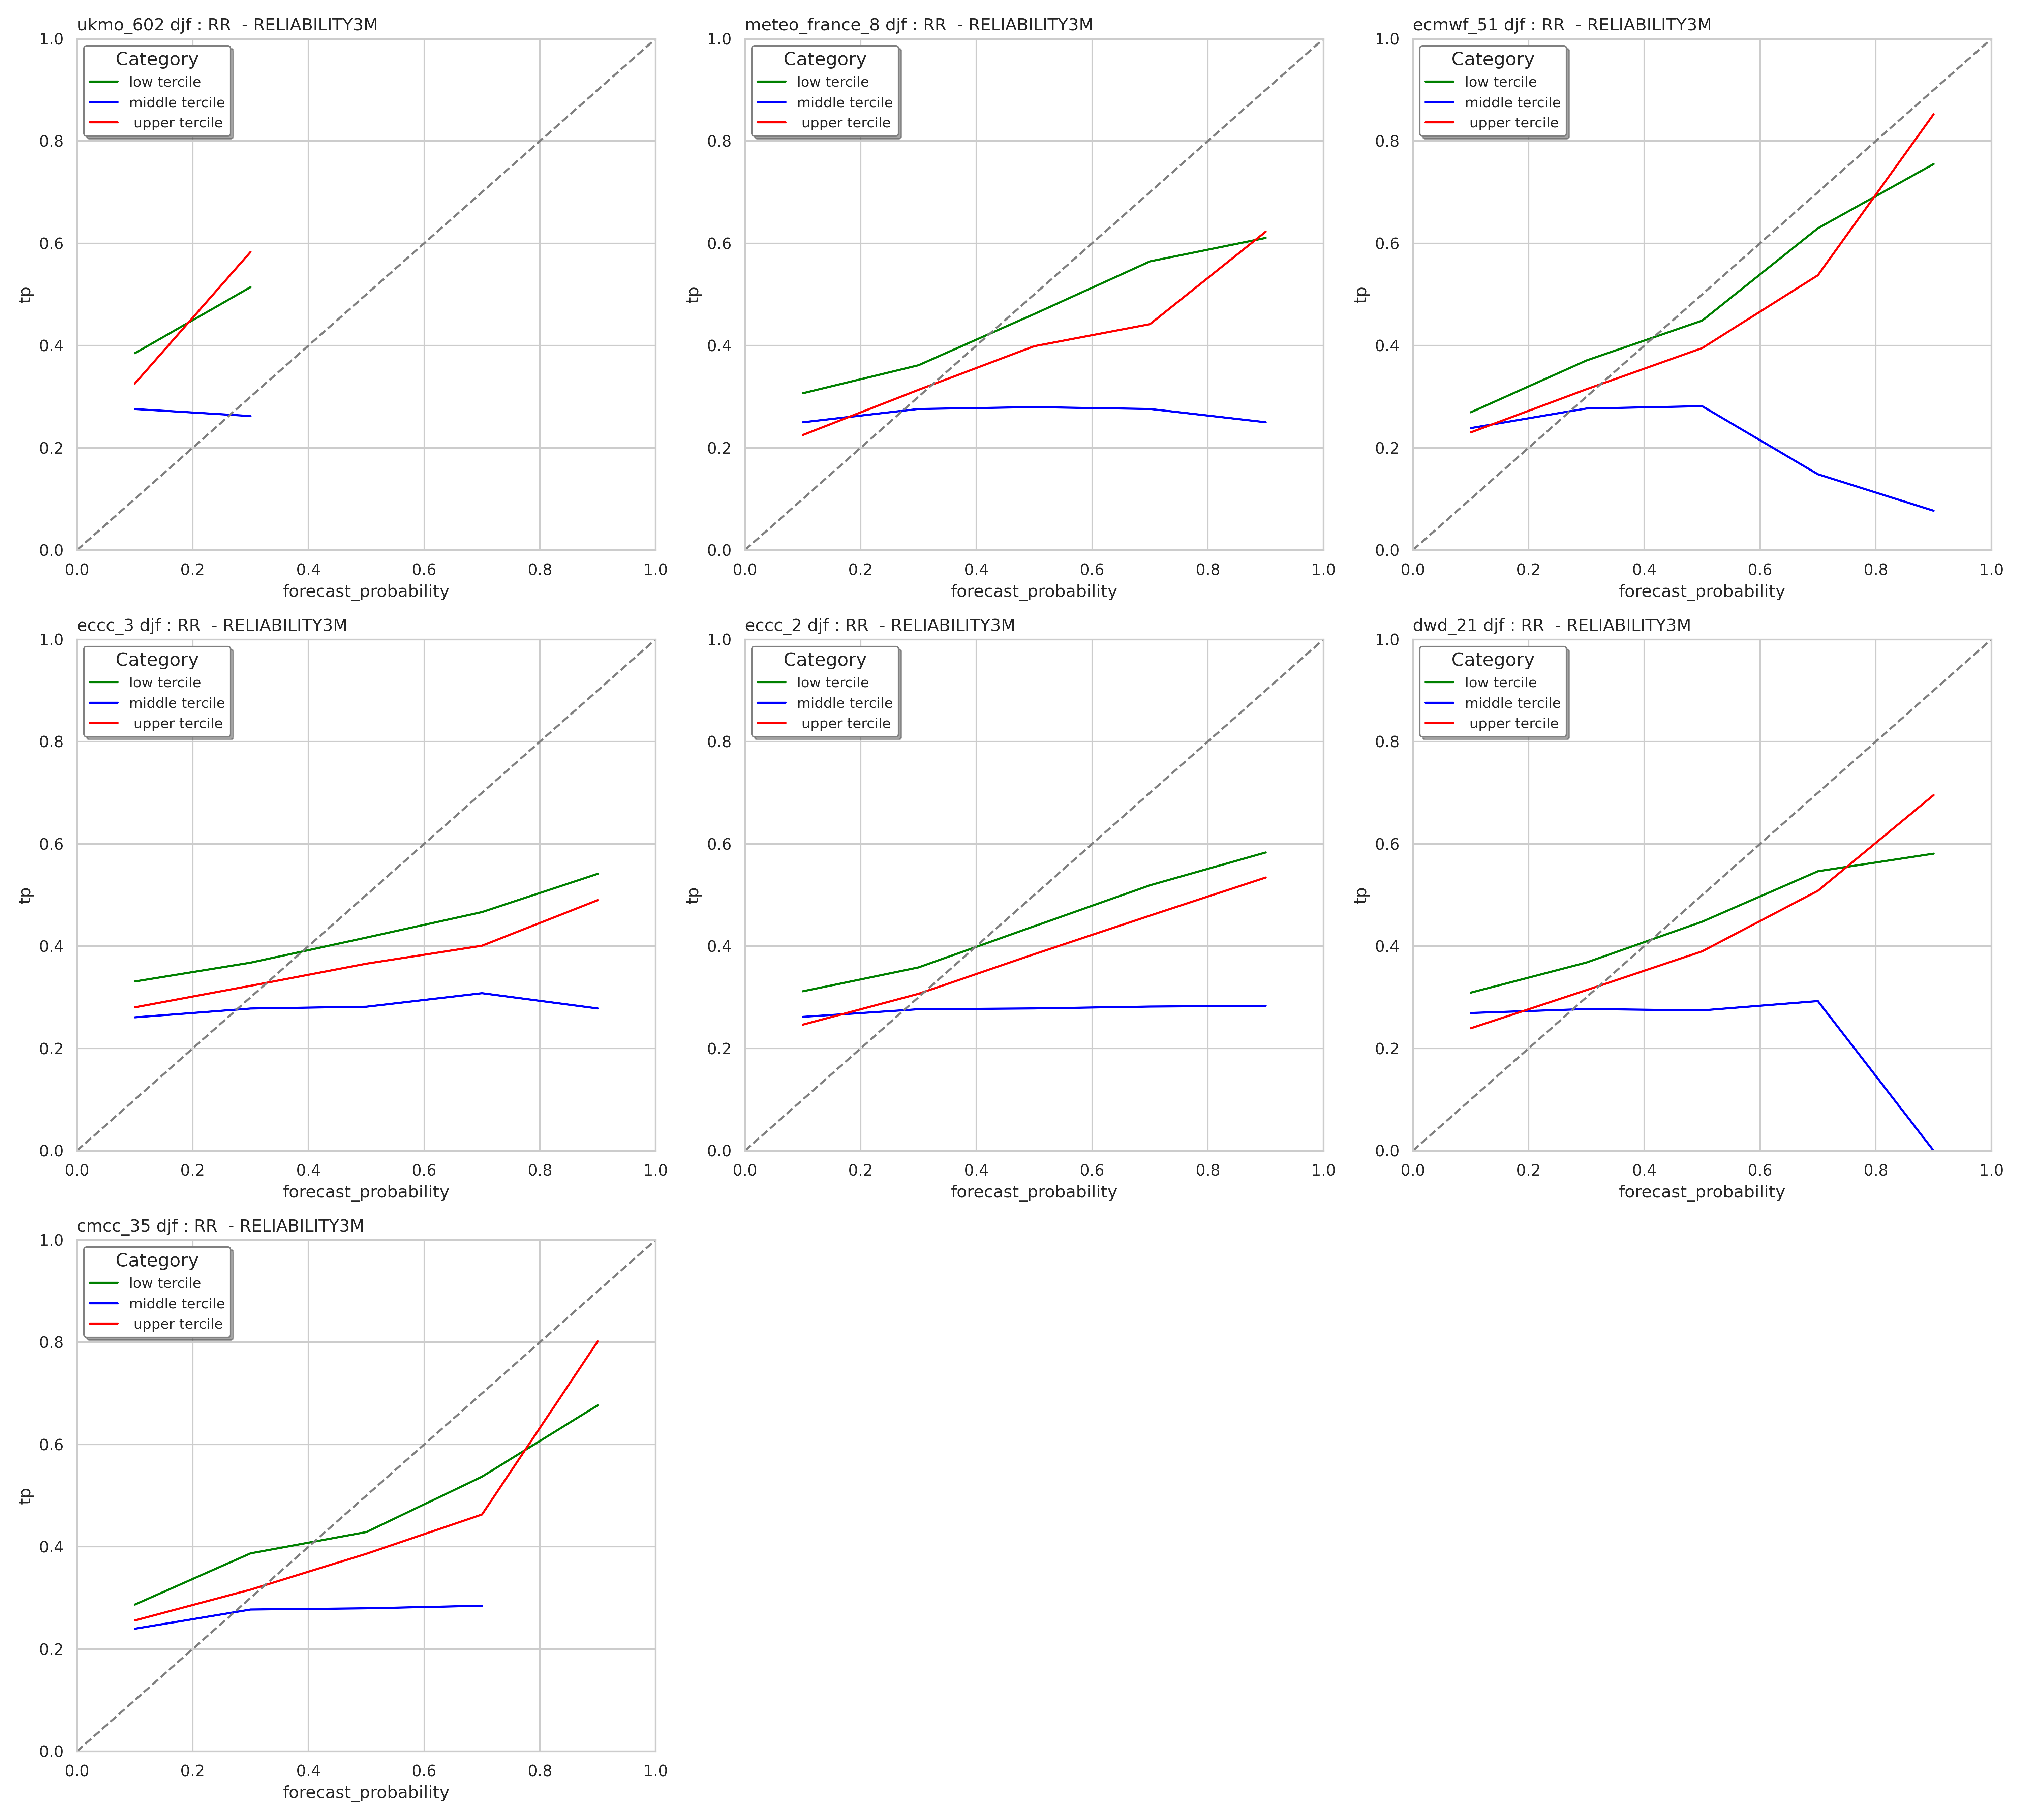
\includegraphics[scale=0.3]{plots/prob/rela/rela_diagram_RR_djf.png}
\caption{The 3-month rolling mean for Reliability DJF   . \textbf{\textit{Reliability is better in cases where the graphs are closer to the 45-degree line}}}
\end{figure}







\subsubsection{The ranked probability score (RPS)}

The Ranked Probability Score (RPS) is a performance metric used in probabilistic forecasting to assess how well the predicted probability distribution matches the observed outcome distribution. It is particularly useful when there are multiple categories (e.g., terciles such as lower, middle, and upper) and is commonly applied in fields such as meteorology, climatology, and economics.

$$RPS=\frac{1}{n(m-1)}\sum\limits_{i=1}^{n} \sum\limits_{k=1}^{m-1} \left(\sum\limits_{j=1}^{k}(y_{j,i} - p_{j,i})\right)^2  $$

where : 

\begin{itemize}
	\item n is the number of forecasts.
	\item m is the number of categories.
	\item $y_{j,i}$ is 1 if the $i^th$ observation was in category j, and is 0 otherwise.
	\item $p_{j,i}$ is the $i^th$ forecast probability for category j
\end{itemize}

The score is the average squared “error” in the cumulative
probabilistic forecasts, and it ranges between 0\% for perfect forecasts (a probability of 100\%
was assigned to the observed category on each forecast) to a maximum of 100\% that can only
be achieved if all the observations are in the outermost categories, and if the forecasts are
perfectly bad (a probability of 100\% was assigned to the opposite outermost category to that
observed).


\begin{figure}[H]
    \centering
    \includegraphics[scale=0.25]{plots/prob/rps/rps_RR.png}
    \caption{The Heatmap of  RPS Score on MENA region for Precipitations    . \textbf{\textit{(0 means perfect RPS)}}}
\end{figure}

In the figure above, all centers demonstrate similar performance, except for UKMO, which shows noticeably lower performance.




\subsubsection{Relative operating characteristics}
The ROC\footnote{wmo guidance verification} can be used in forecast verification to measure \textbf{\textit{the ability of the forecasts to distinguish an event from a non-event}}. For seasonal forecasts with three or more categories, the first
problem is to define the “event”. One of the categories must be selected as the current category
of interest, and an occurrence of this category is known as an event. An observation in any of
the other categories is defined as a non-event and no distinction is made as to which of these
two categories does occur. So, for example, if below normal is selected as the event, normal
and above normal are treated equally as non-events.

the score indicates the probability of successfully
discriminating below-normal observations from normal and above-normal observations. It
indicates how often the forecast probability for below normal is higher when below normal
actually does occur compared to when either normal or above normal occurs.


\begin{figure}[H]
    \centering
    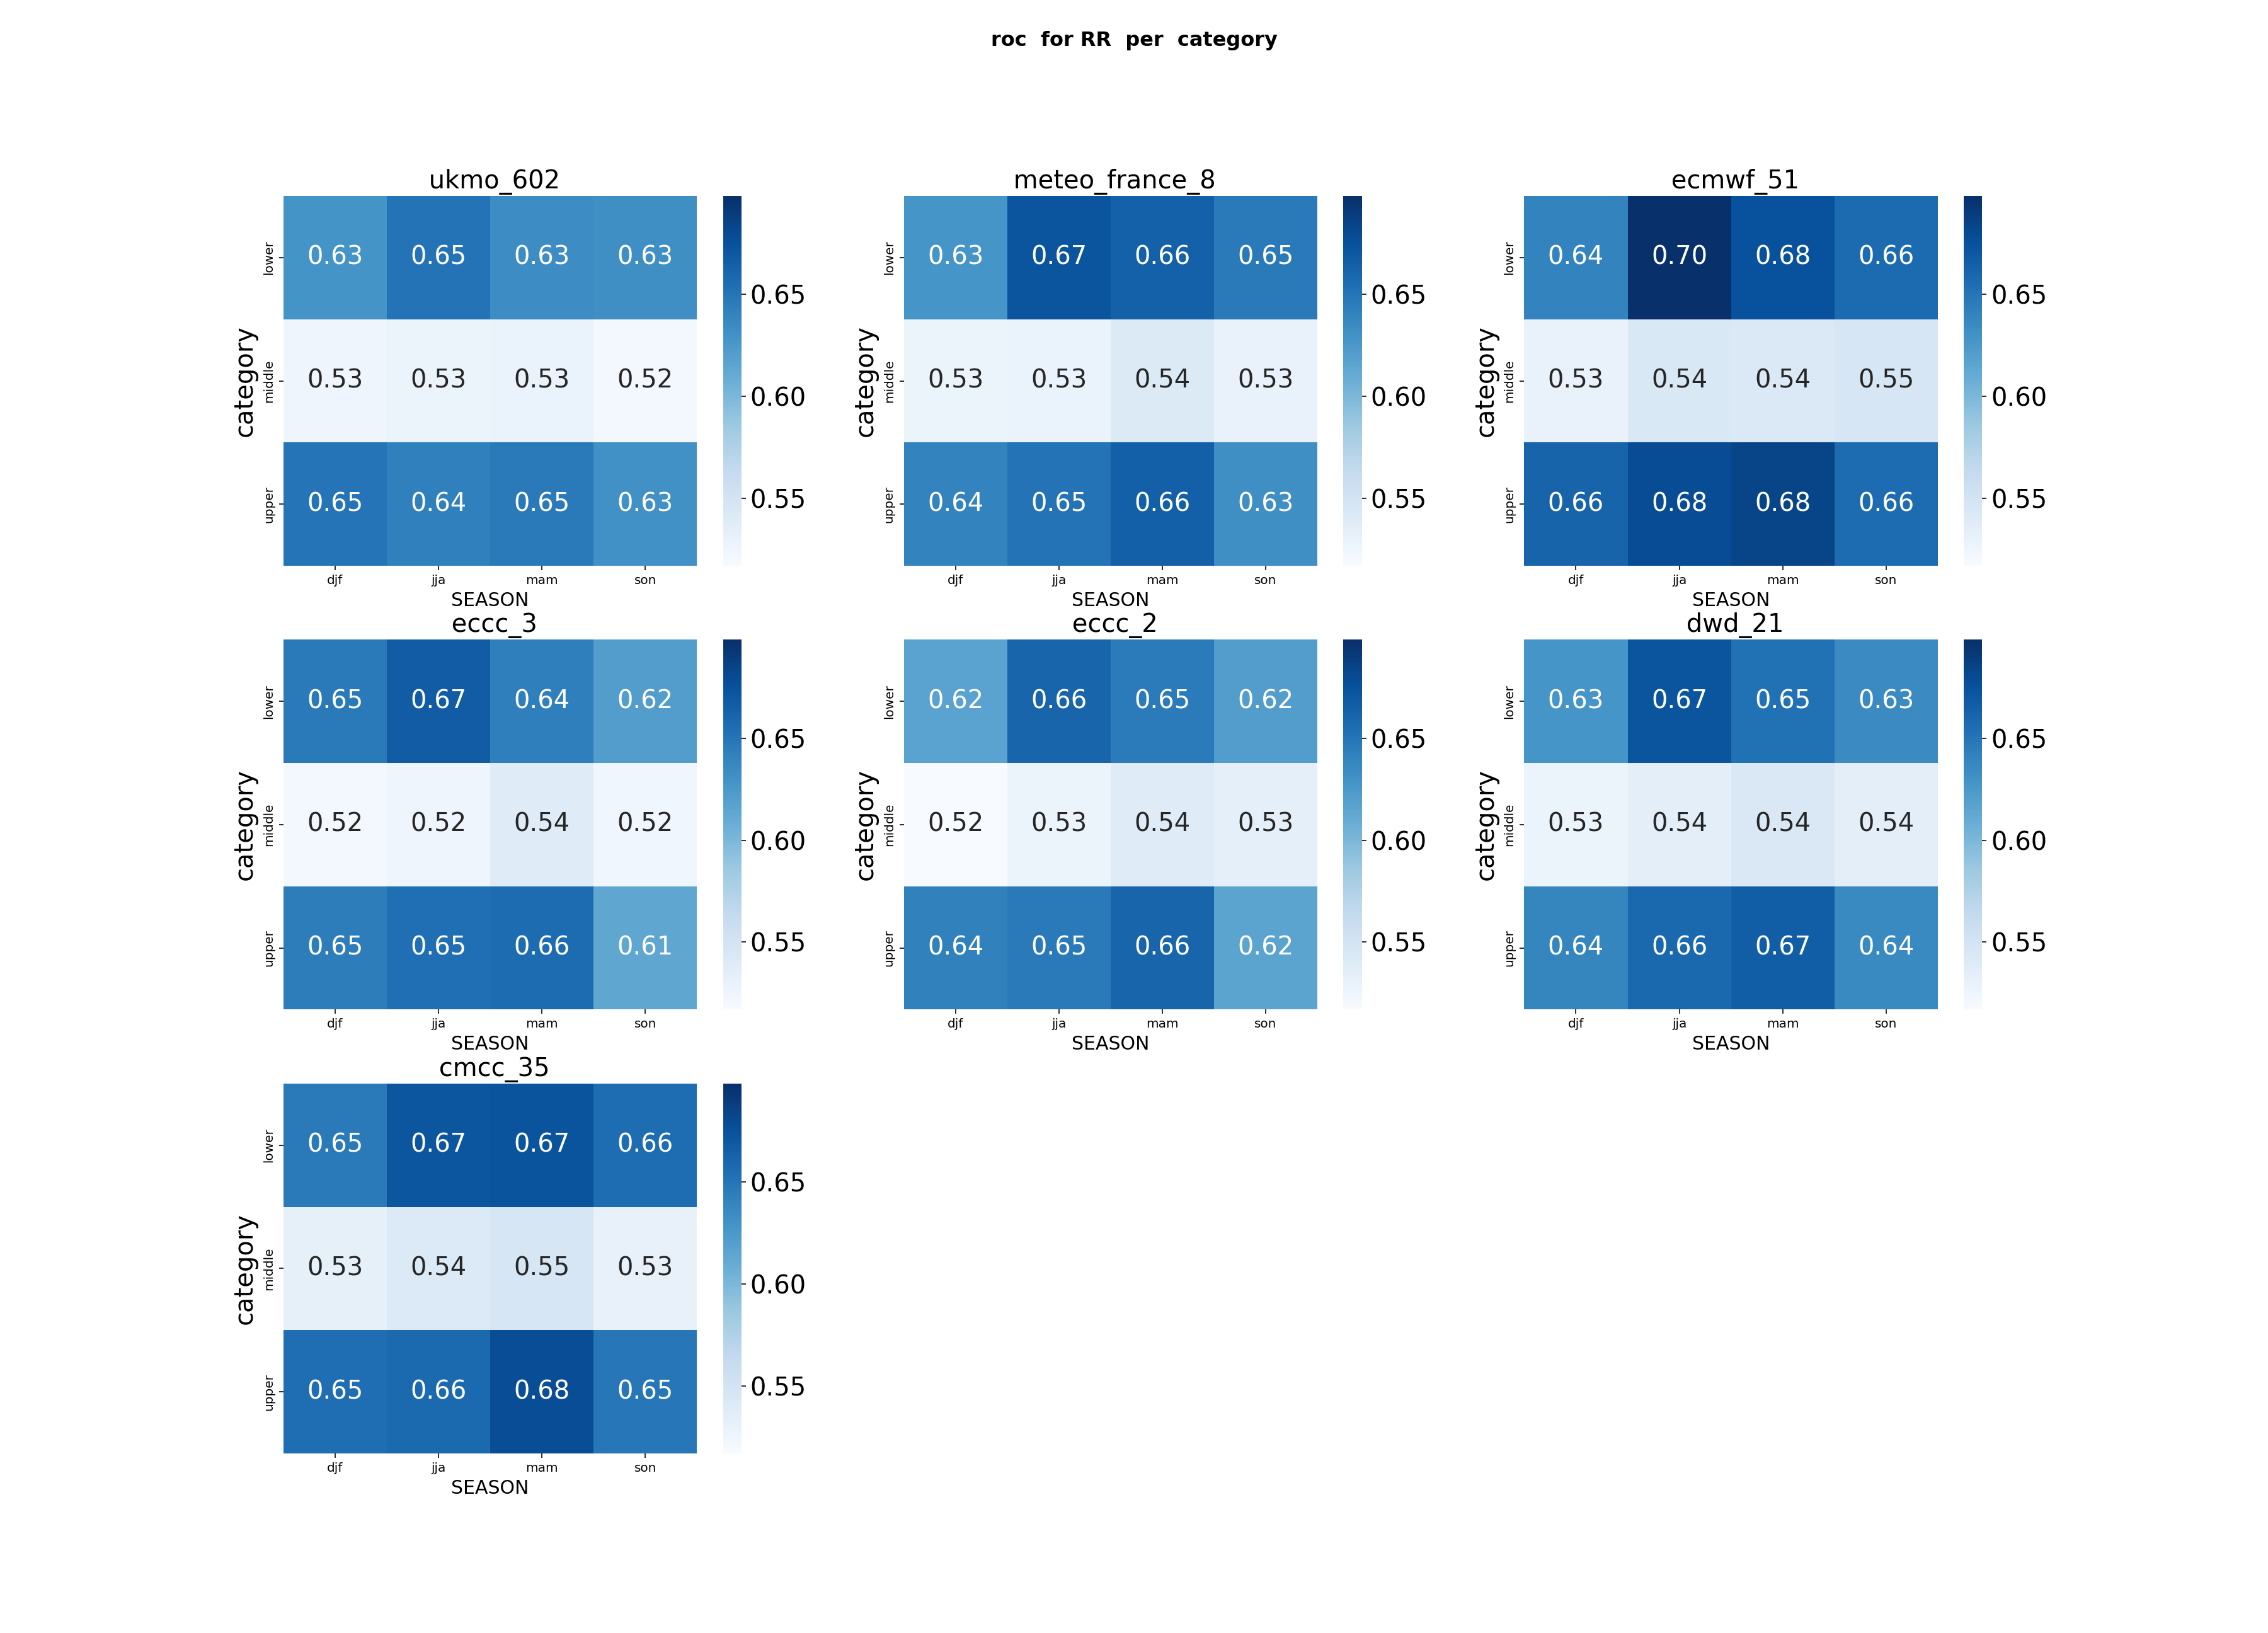
\includegraphics[scale=0.25]{plots/prob/roc/roc_RR_category.png}
    \caption{The Heatmap of ROC Score for each category  . \textbf{\textit{(1 means perfect ROC)}}}
\end{figure}

In the figure above, it is evident that all centers exhibit similar performance levels. However, the middle tercile consistently achieves the lowest score.
\begin{figure}[H]
    \centering
    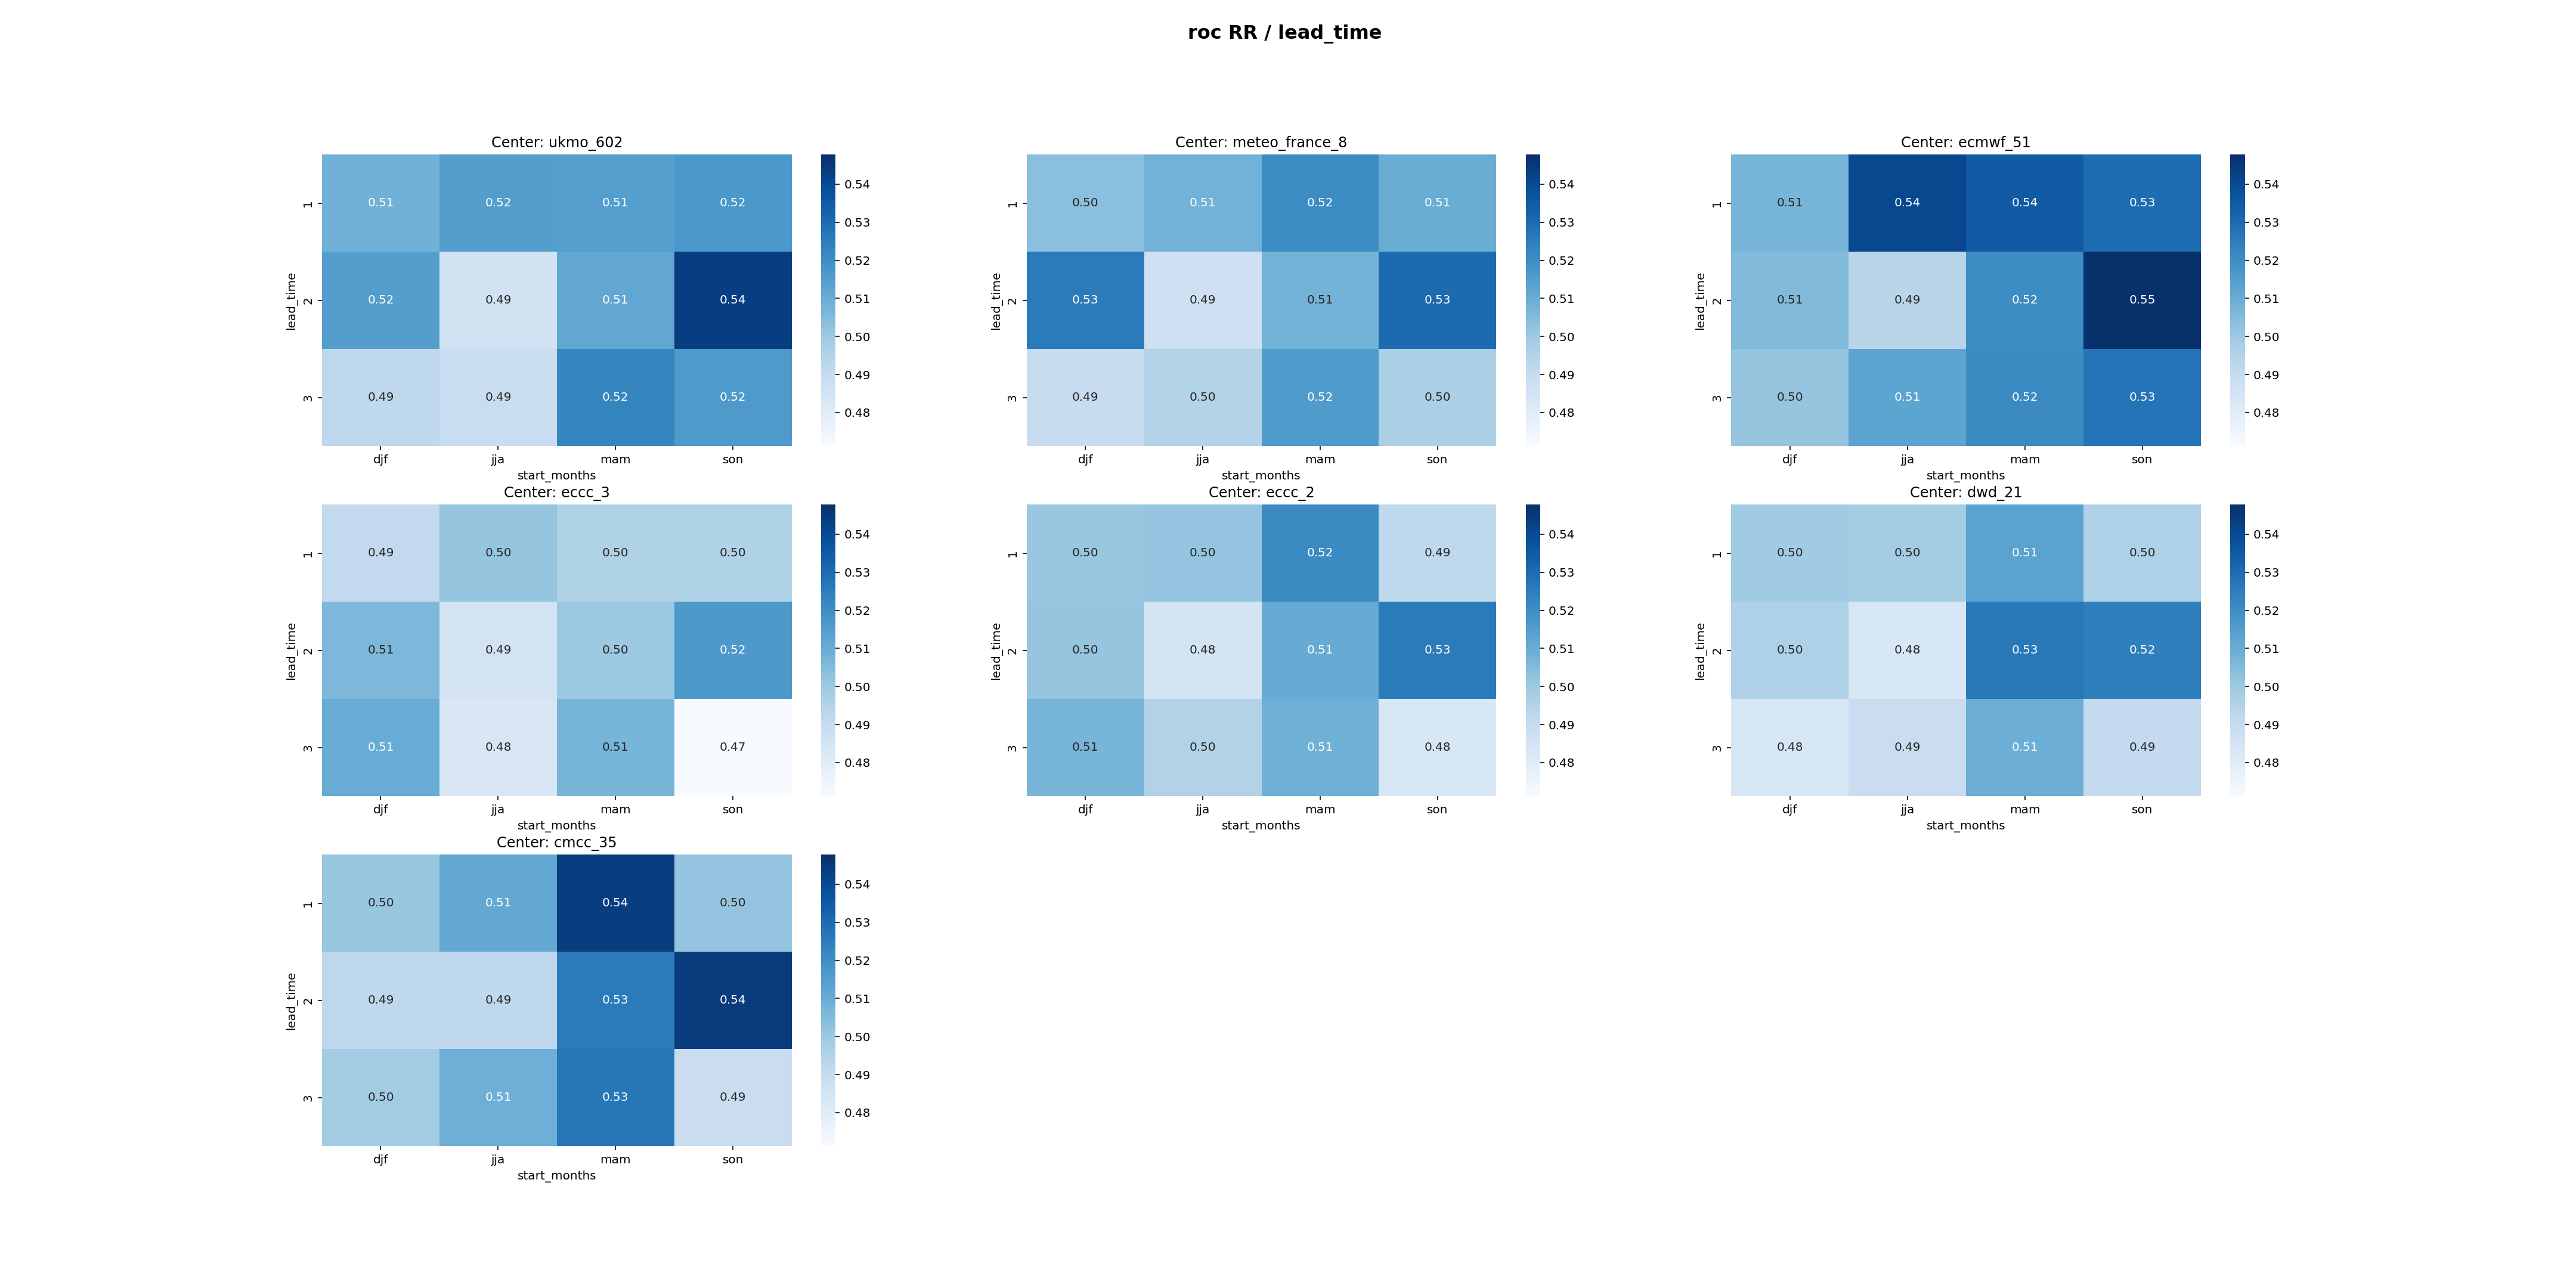
\includegraphics[scale=0.25]{plots/prob/roc/roc_RR_lead_time.png}
    \caption{The Heatmap of ROC Score for lead-times. \textbf{\textit{(1 means perfect ROC)}}}
\end{figure}


\begin{figure}[H]
    \centering
    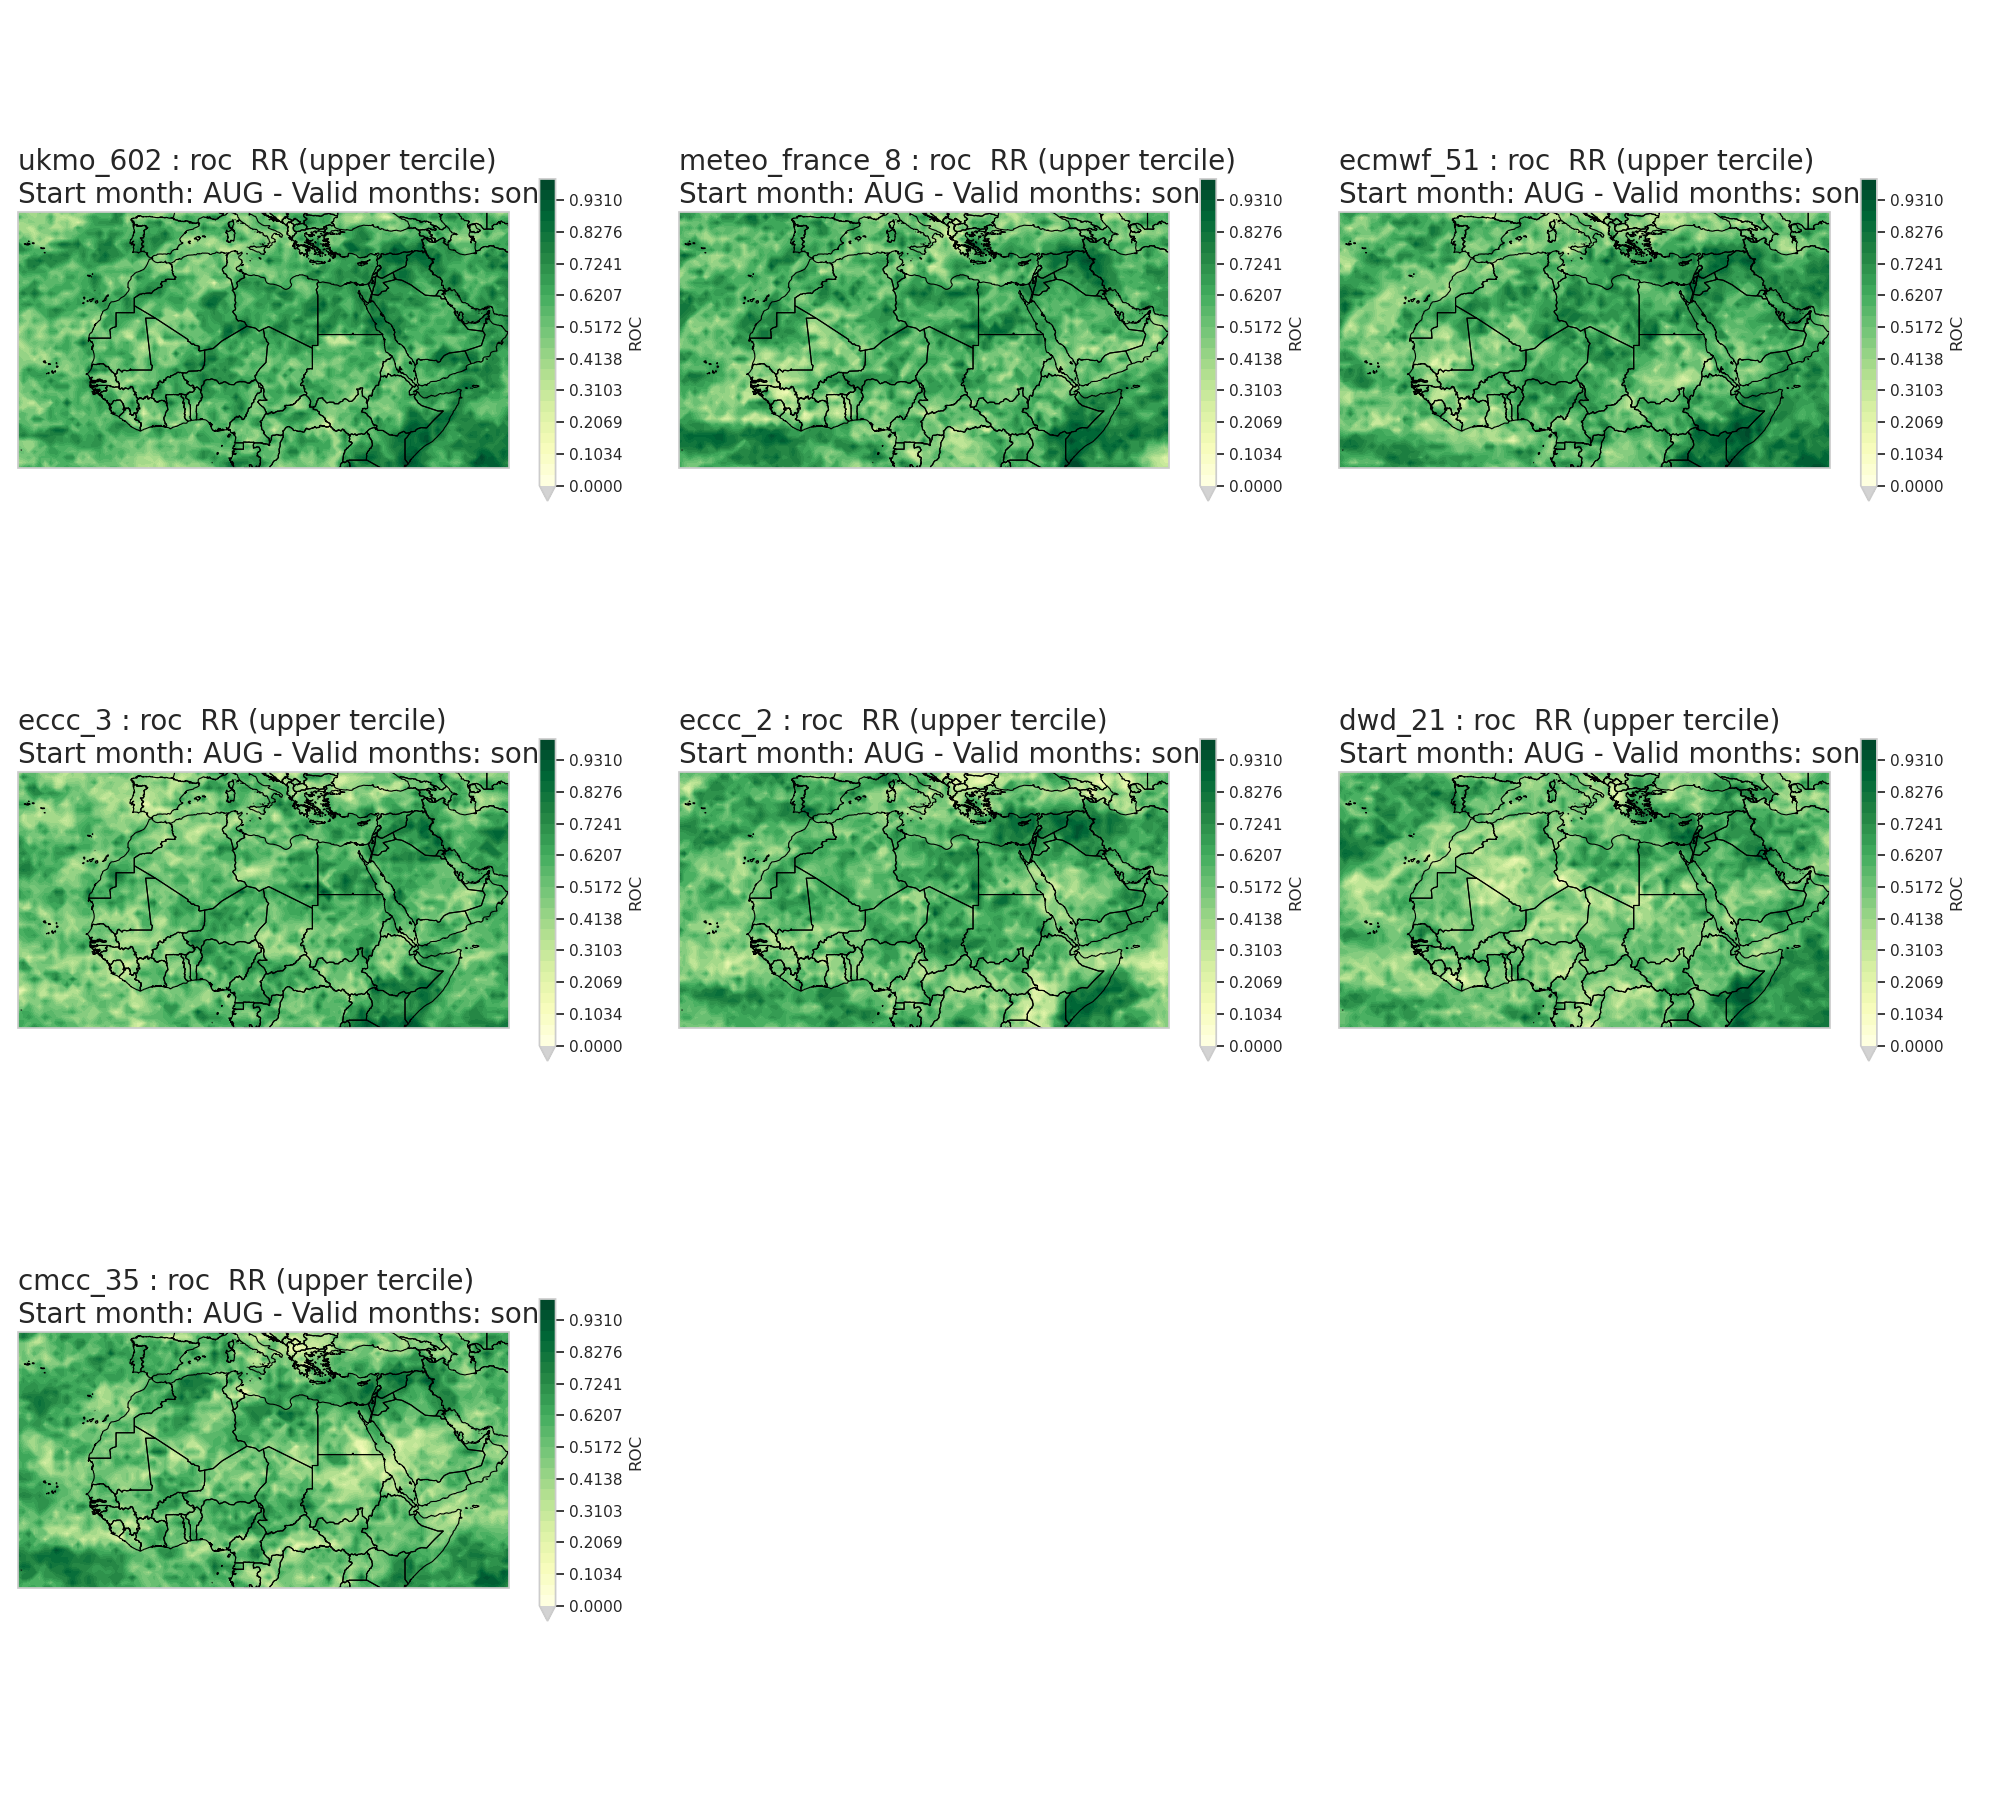
\includegraphics[scale=0.3]{plots/prob/roc/roc_son_RR_upper.png}
    \caption{The ROC Score Upper tercile SON    . \textbf{\textit{(1 means perfect ROC)}}}
\end{figure}


\subsubsection{Relative operating characteristics Skill Score}
The Relative Operating Characteristic Skill Score (ROCSS) is a measure used in forecast verification to assess the ability of probabilistic forecasts to discriminate between events and non-events. It builds on the Relative Operating Characteristic (ROC) curve, which plots the hit rate (true positive rate) against the false alarm rate (false positive rate) at various forecast probability thresholds.

\begin{itemize}
	\item The ROC curve evaluates the discrimination capability of a forecast, i.e., how well the forecast can separate occurrences of an event (e.g., below-normal temperature) from non-events (e.g., normal or above-normal temperature).
	\item The ROC Skill Score quantifies the area under the ROC curve (AUC) and compares it to a no-skill forecast.
\end{itemize}

	$$ROCSS=\frac{AUC-AUC_{no-skill}}{1-AUC_{no-skill}}$$
where:
\begin{itemize}
	\item $AUC$ : Area Under the ROC Curve for the forecast being evaluated.
	\item $AUC_{no-skill}$ : Area Under the Curve for a no-skill forecast 0.5 for our case.
\end{itemize}

Interpretation of ROCSS:
\begin{itemize}
	\item 1: Perfect discrimination ability.
	\item 0: No skill (forecast performs no better than random guessing).
	\item Negative values: Forecast performs worse than random guessing.
\end{itemize}
	

In the figure above, it is evident that the ECMWF exhibit the best performance for all terciles and periods. HOwever, we should notice that the performance is very bad for the middle tercile in all centers.

\begin{figure}[H]
    \centering
    \includegraphics[scale=0.25]{plots/prob/rocss/rocss_RR_category.png}
    \caption{The ROCSS Score for each category  . \textbf{\textit{(1 means perfect ROCSS)}}}
\end{figure}


\begin{figure}[H]
    \centering
    \includegraphics[scale=0.25]{plots/prob/rocss/rocss_RR_lead_time.png}
    \caption{The average of  ROCSS Score on all categories    . \textbf{\textit{(1 means perfect ROCSS)}}}
\end{figure}


\begin{figure}[H]
    \centering
    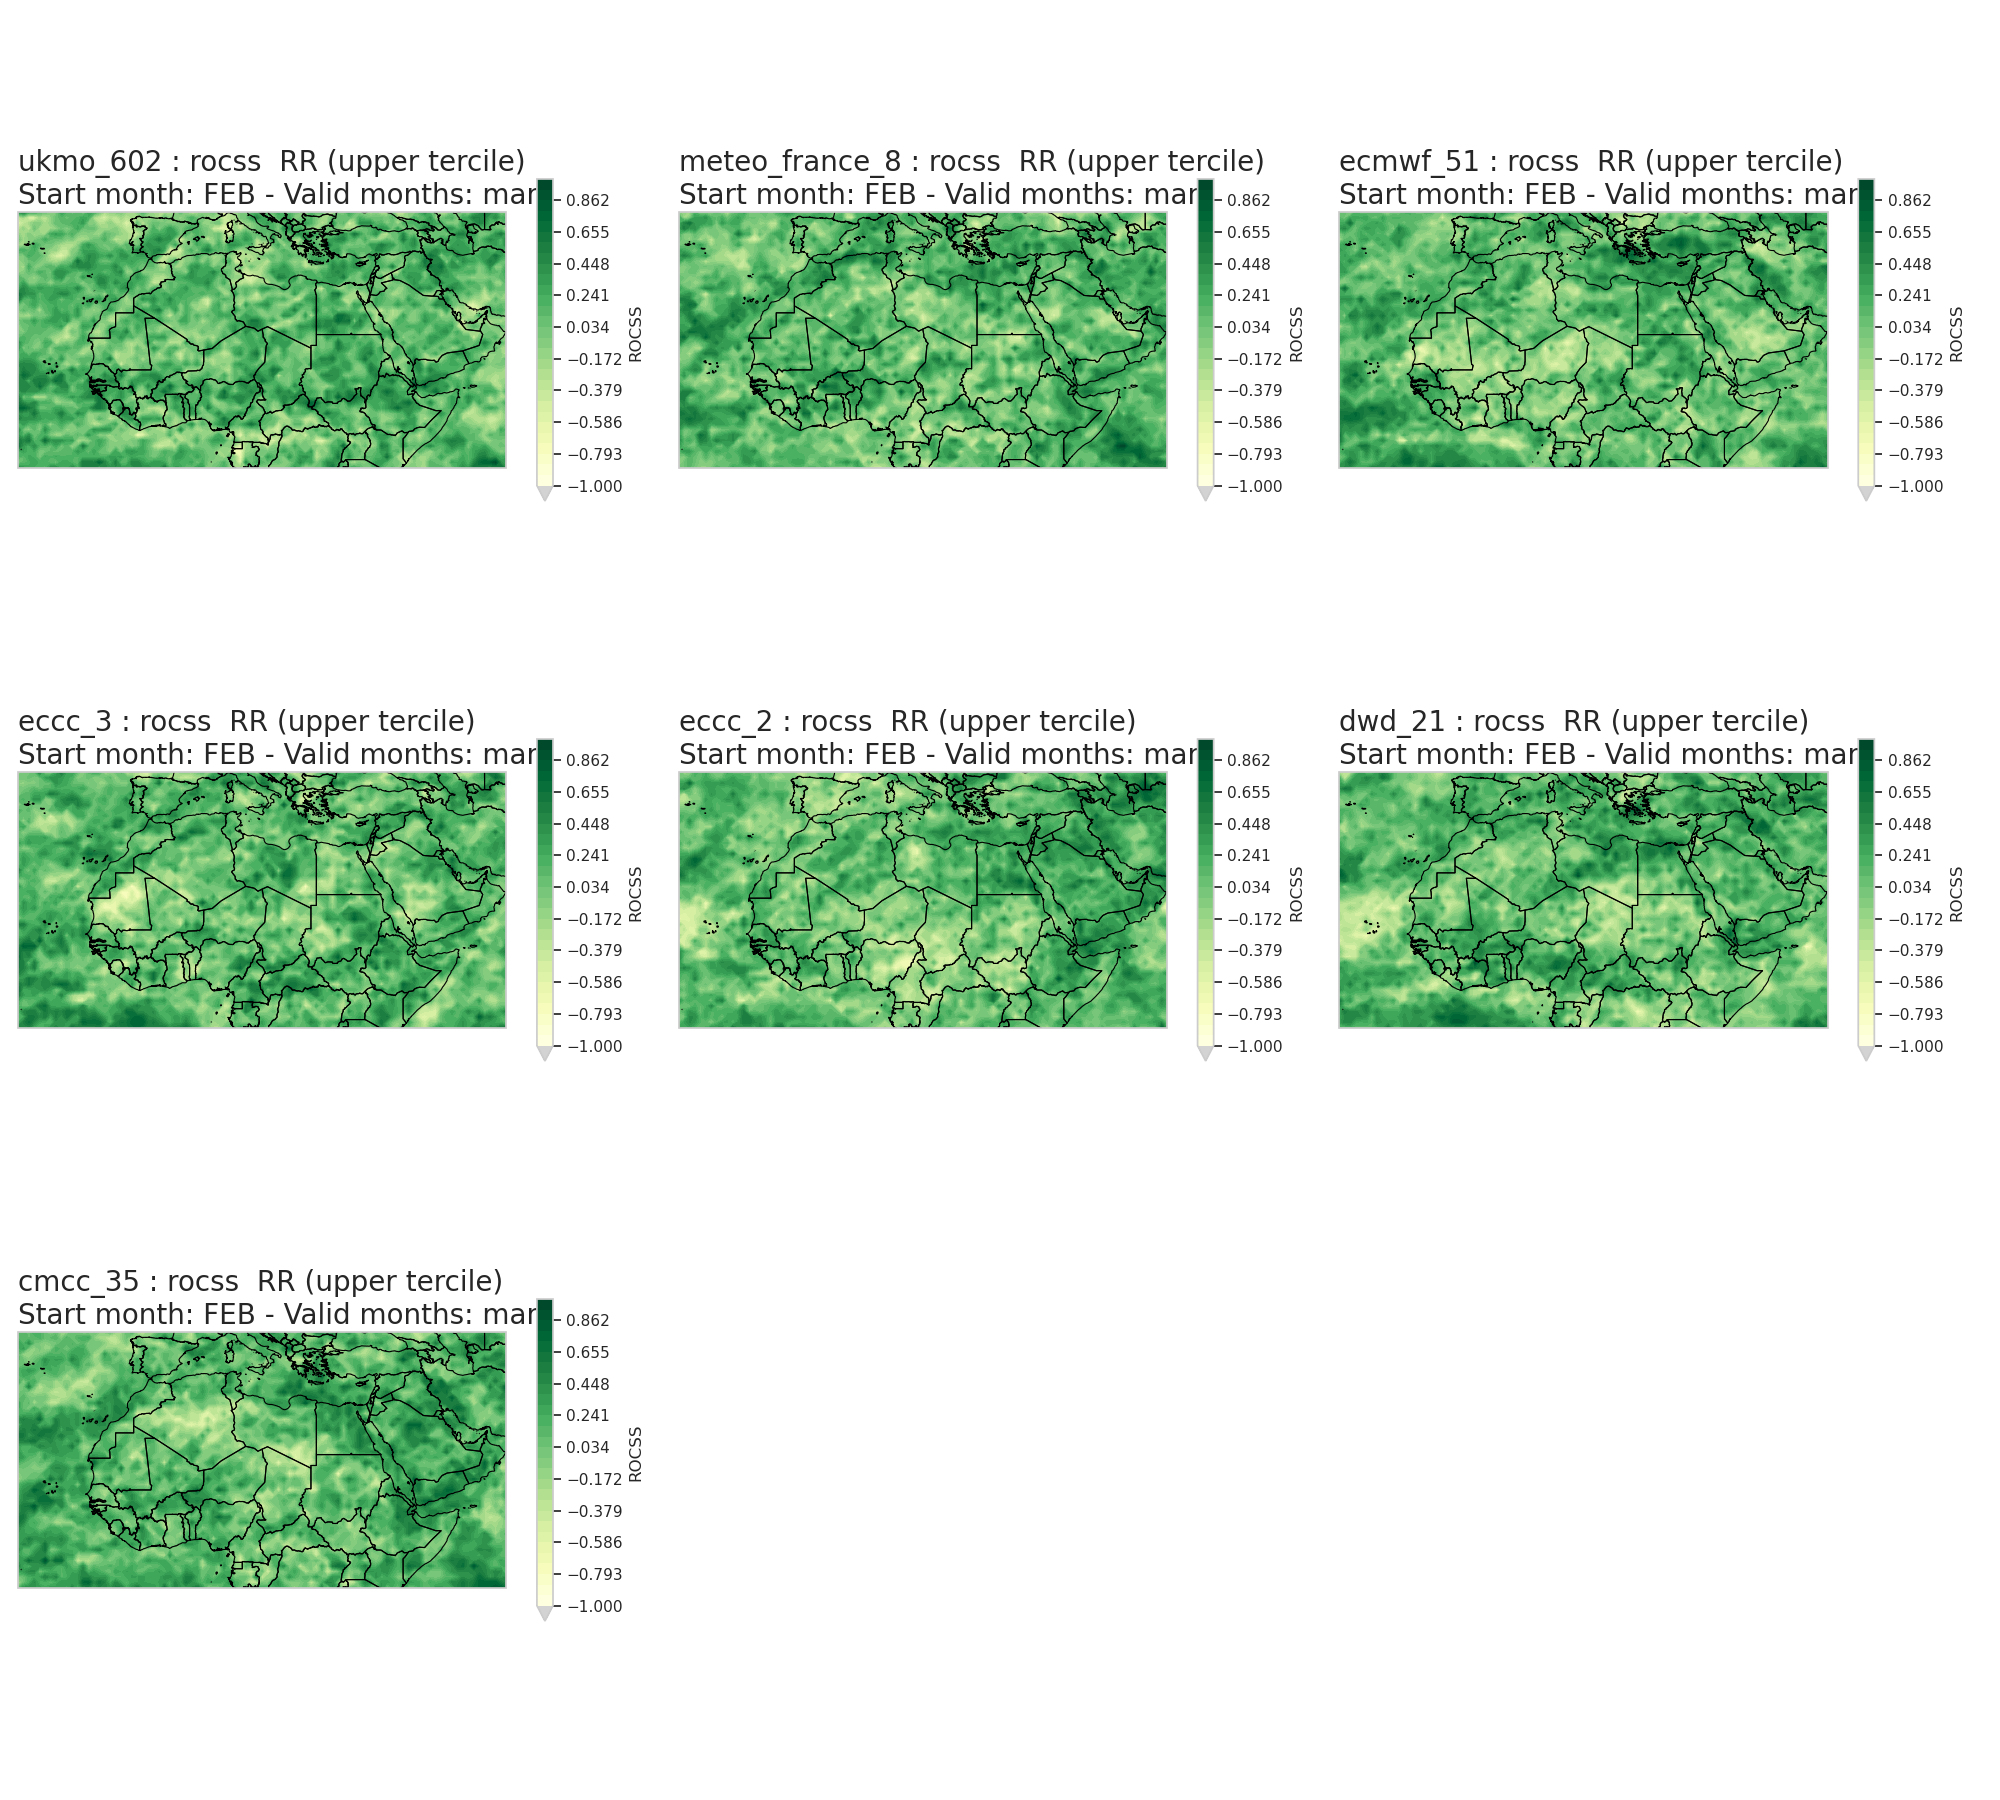
\includegraphics[scale=0.3]{plots/prob/rocss/rocss_mam_RR_upper.png}
    \caption{The ROC Skill Score Upper tercile MAM    . \textbf{\textit{(1 means perfect ROC)}}}
\end{figure}








\subsubsection{summary}
\begin{table}[h!]
\centering
\begin{tabularx}{\textwidth}{@{}p{2.5cm}p{4cm}p{4cm}p{2.5cm}p{3cm}@{}}
\toprule
\textbf{Metric}       & \textbf{Focus}                                    & \textbf{What it Measures}                         & \textbf{Dependent on Observed Outcomes?} & \textbf{Visualization/Tools}             \\ \midrule
\textbf{Reliability}   & Probabilities match observed frequencies          & Calibration of probabilities                      & Yes                                      & Reliability diagram                      \\
\textbf{Discrimination} & Differentiating between outcomes                 & Ability to distinguish events from non-events    & Yes                                      & ROC curve, AUC                           \\
\textbf{Sharpness}     & Boldness of probabilities (away from average)     & Confidence of the forecast                        & No                                       & Histogram of forecast probabilities      \\
\textbf{Resolution}    & Informativeness and variability of forecast       & Ability to provide specific, useful info         & Yes                                      & Brier Score decomposition                \\ \bottomrule
\end{tabularx}
\caption{Key differences between reliability, discrimination, sharpness, and resolution in seasonal forecasting.}
\label{tab:forecast_metrics}
\end{table}

\newpage
\thispagestyle{empty}
\mbox{}